\documentclass[12pt]{article}
\usepackage{multirow}
\usepackage{caption}
\usepackage{bm}
\usepackage{amsmath}
\usepackage{amsfonts}
\usepackage{amssymb}
\usepackage{graphicx}
\usepackage{colortbl}
\usepackage{xr}
\usepackage{hyperref}
\usepackage[all]{hypcap} 
\usepackage{longtable}
\usepackage{xfrac}
\usepackage{tabularx}
\usepackage{float}
\usepackage{siunitx}
\usepackage{booktabs}
\usepackage[toc, page]{appendix}
\usepackage{url}
\usepackage[usenames,dvipsnames]{xcolor}
\usepackage{array}
\usepackage{tabu}
\usepackage[numbib,nottoc]{tocbibind}
%\usepackage{refcheck}

\hypersetup{
      colorlinks=true,       % false: boxed links; true: coloured links
      linkcolor=red,          % colour of internal links (change box colour with
                              % %linkbordercolor)
    citecolor=blue,        % colour of links to bibliography
    filecolor=magenta,      % colour of file links
    urlcolor=cyan           % colour of external links
}

%% Comments
\newif\ifcomments\commentstrue

\ifcomments
\newcommand{\authornote}[3]{\textcolor{#1}{[#3 ---#2]}}
\newcommand{\todo}[1]{\textcolor{red}{[TODO: #1]}}
\else
\newcommand{\authornote}[3]{}
\newcommand{\todo}[1]{}
\fi

\newcommand{\wss}[1]{\authornote{magenta}{SS}{#1}}
\newcommand{\nk}[1]{\authornote{blue}{NK}{#1}}

\newcommand{\colZwidth}{1.0\textwidth}
\newcommand{\blt}{- } %used for bullets in a list
\newcommand{\colAwidth}{0.13\textwidth}
\newcommand{\colBwidth}{0.82\textwidth}
\newcommand{\colCwidth}{0.1\textwidth}
\newcommand{\colDwidth}{0.05\textwidth}
\newcommand{\colEwidth}{0.8\textwidth}
\newcommand{\colFwidth}{0.17\textwidth}
\newcommand{\colGwidth}{0.5\textwidth}
\newcommand{\colHwidth}{0.28\textwidth}
\newcounter{defnum} %Definition Number
\newcommand{\dthedefnum}{GD\thedefnum}
\newcommand{\dref}[1]{GD\ref{#1}}
\newcounter{datadefnum} %Datadefinition Number
\newcommand{\ddthedatadefnum}{DD\thedatadefnum}
\newcommand{\ddref}[1]{DD\ref{#1}}
\newcounter{theorynum} %Theory Number
\newcommand{\tthetheorynum}{T\thetheorynum}
\newcommand{\tref}[1]{T\ref{#1}}
\newcounter{tablenum} %Table Number
\newcommand{\tbthetablenum}{T\thetablenum}
\newcommand{\tbref}[1]{TB\ref{#1}}
\newcounter{assumpnum} %Assumption Number
\newcommand{\atheassumpnum}{P\theassumpnum}
\newcommand{\aref}[1]{A\ref{#1}}
\newcounter{physsysnum} %Physical System Description Number
\newcommand{\pthephyssysnum}{P\thephyssysnum}
\newcommand{\psref}[1]{PS\ref{#1}}
\newcounter{goalnum} %Goal Number
\newcommand{\gthegoalnum}{P\thegoalnum}
\newcommand{\gsref}[1]{GS\ref{#1}}
\newcounter{instnum} %Instance Number
\newcommand{\itheinstnum}{IM\theinstnum}
\newcommand{\iref}[1]{IM\ref{#1}}
\newcounter{reqnum} %Requirement Number
\newcommand{\rthereqnum}{P\thereqnum}
\newcommand{\rref}[1]{R\ref{#1}}
\newcounter{lafnum}
\newcommand{\lthelafnum}{L\thelafnum}
\newcommand{\lref}[1]{L\laf{#1}}
\newcounter{uahnum}
\newcommand{\utheuahnum}{U\theuahnum}
\newcommand{\uref}[1]{U\uaf{#1}}
\newcounter{perfnum}%Appendix
\newcommand{\ptheperfnum}{AP\theperfnum}
\newcommand{\perf}[1]{AP\perf{#1}}
\newcounter{oaenum}
\newcommand{\otheoaenum}{O\theoaenum}
\newcommand{\oae}[1]{P\oae{#1}}
\newcounter{masnum}
\newcommand{\mthemasnum}{M\themasnum}
\newcommand{\mas}[1]{P\mas{#1}}
\newcounter{secunum}
\newcommand{\sthesecunum}{S\thesecunum}
\newcommand{\secu}[1]{S\secu{#1}}
\newcounter{culnum}
\newcommand{\ctheculnum}{C\theculnum}
\newcommand{\cul}[1]{P\cul{#1}}
\newcounter{apnum}
\newcommand{\atheapnum}{L\theapnum}
\newcommand{\apref}[1]{AP\ap{#1}}

\newcounter{lcnum} %Likely change number
\newcommand{\lthelcnum}{LC\thelcnum}
\newcommand{\lcref}[1]{LC\ref{#1}}

\newcounter{ucnum} %Unlikely change number
\newcommand{\utheucnum}{UC\theucnum}
\newcommand{\ucref}[1]{UC\ref{#1}}

\newcommand{\tclad}{T_\text{CL}}
\newcommand{\degree}{\ensuremath{^\circ}}
\newcommand{\progname}{GlassBR}
\newcommand{\euler}{e}
\newcommand{\complex}{i}

\newcolumntype{P}[1]{>{\centering\arraybackslash}p{#1}}

\oddsidemargin 0mm
\evensidemargin 0mm
\textwidth 160mm
\textheight 200mm
%\usepackage{fullpage}

\begin{filecontents}{../../refs/References.bib}
\end{filecontents}

\begin{document}

\title{Software Requirements Specification for \progname} 
\author{Nikitha Krishnan and W. Spencer Smith}
\date{\today}

\maketitle

\tableofcontents
\newpage

\section{Reference Material}

This section records information for easy reference.

\subsection{Table of Units}

The unit system used throughout is SI (Syst\`{e}me International d'Unit\'{e}s). In addition to the
basic units, several derived units are also used. For each unit, the table lists the symbol, a
description and the SI name.
~\newline

\renewcommand{\arraystretch}{1.2}
  \noindent \begin{tabular}{l l l} 
    \toprule		
    \textbf{Symbol} & \textbf{Description} & \textbf{SI}\\
    \midrule 
    \si{\kilogram} & mass & kilogram\\	
    \si{\meter} & distance & metre\\	
    \si{\newton} & force & newton\\	
    \si{\pascal} & pressure & pascal\\
    \si{\second} & time & second\\	
    \bottomrule
  \end{tabular}
  %	\caption{Provide a caption}

\subsection{Table of Symbols}\label{TblSym}

The table that follows summarizes the symbols used in this document along with 
their units.  The symbols are listed in alphabetical order.
\newline
% \wss{The table of symbols should be checked, and it should be sorted into
%   alphabetical order.  Do not include symbols that are not used.}

\renewcommand{\arraystretch}{1.2}

\noindent 
\begin{longtable}{l l p{12cm}} \toprule
  \textbf{Symbol} & \textbf{Unit} & \textbf{Description}\\
  \midrule
  %$\gamma$& -- & Shear transfer coefficient\\
  %$A$ & \si{\milli\meter ^2} & Area of glass plate\\
  $a$ &  \si{\meter} & Plate length (long dimension)\\
  $\text{AR} $ & -- & Aspect ratio\\
  $\text{AR}_{\text{max}} $ & -- & Maximum aspect ratio\\
  $b$& \si{\meter}        & Plate width (short dimension)\\
  $B$ & -- & Risk function\\
  $d_{\text{max}} $& \si{\meter} & Maximum value for one of the dimensions of the glass plate\\
  $d_{\text{min}} $& \si{\meter} & Minimum value for one of the dimensions of the glass plate\\
  $E$ & \si{\pascal} & Modulus of elasticity of glass\\
  $g$ & -- & Glass type, $g \in \{ \text{AN}, \text{HS}, \text{FT} \}$\\
  $\text{GTF} $ & -- & Glass type factor\\
  $h$ & \si{\meter} & Minimum thickness\\
  $\text{is\_safe1}$ & -- & Variable that is assigned true when calculated probability is less than
                                  tolerable probability\\
  $\text{is\_safe2}$ & -- & Variable that is assigned true when load resistance (capacity) is
                                  greater than load (demand)\\
  $J$ & -- & Stress distribution factor (Function)\\
  $J_{\text{tol}}$ & -- & Stress distribution factor (Function) based on $P_{b_{\text{tol}}}$\\
  $k$ & \si{\newton ^{-7}\meter ^{12} } & Surface flaw parameter\\
  $\text{LDF} $ & -- & Load duration factor\\
  $\text{LR} $ & -- & Load resistance\\
  $\text{LSF} $ & -- & Load share factor\\
  $m$ &  \si{\newton ^{-7}\meter ^{12} } & Surface flaw parameter\\
  $\text{NFL} $ & -- & Non-factored load\\
  $P_b$ & -- &  Probability of breakage\\
  $P_{b_{\text{tol}}}$ & -- &  Tolerable probability of breakage\\
  $q$ & \si{\pascal} & Applied load (demand)\\
  $\hat{q}$ & -- & Dimensionless load\\
  $\hat{q}_{\text{tol}}$ & -- & Tolerable load\\  
  $\text{SD}$ & \si{\meter} & Stand off distance which is represented in
                              coordinates $(\text{SD}_x , \text{SD}_y ,
                              \text{SD}_z)$\\
  $\text{SD}_{\text{max}} $ & \si{\meter} & Maximum stand off distance
                                            permissible for input\\
  $\text{SD}_{\text{min}} $ & \si{\meter} & Minimum stand off distance
                                            permissible for input\\
  $\text{SD}_{\text{x}} $ & \si{\meter} & Stand off distance (x-component)\\
  $\text{SD}_{\text{y}} $ & \si{\meter} & Stand off distance (y-component)\\  
  $\text{SD}_{\text{z}} $ & \si{\meter} & Stand off distance (z-component)\\
  $t$ & \si{\milli\meter} &  Nominal thickness \\
      &                   &  $t \in
                            \{2.5, 2.7, 3.0, 4.0, 5.0, 6.0, 8.0, 10.0,
                            12.0, 16.0, 19.0, 22.0\}$\\
  $t_d$ & s & Duration of load\\
  $\text{TNT} $ & -- & TNT equivalent factor\\
  $w$ & \si{\kilo\gram} & Charge weight\\
  $w_{\text{max}}$ & \si{\kilo\gram} & Maximum permissible input charge weight\\
  $w_{\text{min}}$ & \si{\kilo\gram} & Minimum permissible input charge weight\\
  $w_{\text{TNT}}$& \si{\kilo\gram} & Explosive mass in equivalent weight of TNT\\
  \bottomrule
\end{longtable}

\subsection{Abbreviations and Acronyms}

~\newline \renewcommand{\arraystretch}{1.2}
\noindent 
\begin{tabular}{l l } \toprule
  \textbf{Abbreviation} & \textbf{Full Form}\\
  \midrule
  A & Assumption\\
  AN & Annealed\\
  AR & Aspect Ratio\\
  DD & Data Definition\\
  FT & Fully Tempered\\
  GS & Goal Statement\\
  GTF & Glass Type Factor\\
  HS & Heat Strengthened \\
  IG & Insulating Glass \\
  IM & Instance Model\\
  LC & Likely Change\\
  LG & Laminated Glass\\
  N/A & Not Applicable\\
  PS & Physical System Description\\
  R & Requirement\\
  SD & Stand Off Distance\\
  SRS & 	Software Requirements Specification\\
  T & Theoretical Model\\
  UC & Unlikely Change\\
  % SDF & Stress Distribution Factor \\
  % $\text{SDF}_{\text{tol}}$ & Stress Distribution Factor with respect to
  % $P_{b_{\text{tol}}}$\\
  \bottomrule
\end{tabular}

\section{Introduction}

Software is helpful to efficiently and correctly predict the blast risk involved
with the glass slab. The blast under consideration is any type of man-made
explosion. The software, herein called \progname, aims to predict the blast risk
involved with the glass slab using an intuitive interface.  

The following section provides an overview of the Software Requirements Specification (SRS)
for \progname.  This section explains the purpose the document, the scope of 
the system, the organization of the document, and the characteristics of 
the intended reader.

\subsection{Purpose of Document}

The main purpose of this document is to predict whether a given glass slab is
likely to resist a specified blast.  The goals and theoretical models used in
the \progname{} code are provided, with an emphasis on explicitly identifying
assumptions and unambiguous definitions.  This document is intended to be used
as a reference to provide all information necessary to understand and verify the
analysis.  The SRS is abstract because the contents say \emph{what} problem is
being solved, but not \emph{how} to solve it.

This document will be used as a starting point for subsequent development
phases, including writing the design specification and the software verification
and validation plan.  The design document will show how the requirements are to
be realized, including decisions on the numerical algorithms and programming
environment.  The verification and validation plan will show the steps that will
be used to increase confidence in the software documentation and the
implementation. Although the SRS fits
in a series of documents that follow the so-called waterfall model, the actual development
process is not constrained in any way. Even when the waterfall model is not followed, as
Parnas and Clements point out \cite{ParnasAndClements1986}, the most logical way to present
the documentation is still to ``fake" a rational design process.

\subsection{Scope of Requirements} 

The scope of the requirements includes getting all input parameters related to
the glass slab and also the parameters related to blast type. Given the appropriate inputs,
\progname{} predicts whether a glass slab is safe or not.

\subsection{Characteristics of Intended Reader}
\label{Sec:CharofInteRead}
Reviewers of this documentation should have a strong knowledge in theory behind
glass breakage and blast risk. The reviewers should also have an understanding
of second year calculus, structural mechanics, and computer applications in
civil engineering. In addition, reviewers should be familiar with the applicable
standards for constructions using glass \cite{ASTM2009, ASTM2016,
  ASTM2012a}. The users of \progname{} can have a lower level of expertise, as
explained in Section~\ref{sec_userchar}.

\subsection{Organization of Document}

The organization of this document follows the template for an SRS for scientific
computing software proposed by~\cite{Koothoor2013} and \cite{SmithAndLai2005},
with some aspects taken from Volere template 16
\cite{RobertsonAndRobertson1999Vol}. The presentation follows the standard
pattern of presenting goals, theories, definitions, and assumptions.  For
readers who would like a more bottom up approach, they can start reading the
data definitions in Section \ref{sec_datadef} and trace back to find any
additional information they require.

The goal statements are refined to the theoretical models, and theoretical
models to the instance models. The data definitions are used to support the
definitions of the different models.

\section{Stakeholders}

This section describes the stakeholders: the people who have an interest in the
product.

\subsection{The Client}

The client for \progname{} is a company named Entuitive. It is developed by
Dr.\ Manuel Campidelli. The client has the final say on acceptance of the product.

\subsection{The Customer}

The customers are the end users of \progname{}.

\section{General System Description}

This section provides general information about the system including identifying
the interfaces between the system and its environment (system context), describing
the user characteristics and listing the system constraints.

\subsection{System Context}

Figure~\ref{Fig_SystemContext} shows the system context.  A circle represents an
external entity outside the software, the user in this case.  A rectangle
represents the software system itself (\progname{}).  Arrows are used to show the data
flow between the system and its environment.

\begin{figure}[h!]
	\begin{center}
		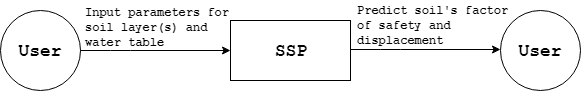
\includegraphics[width=0.6\textwidth]{SystemContextFigure.png}
		\caption{System Context}
		\label{Fig_SystemContext} 
	\end{center}
\end{figure}

The interaction between the product and the user is through a user
interface.  The responsibilities of the user and the system are as follows:

\begin{itemize}
\item User Responsibilities:
  \begin{itemize}
  \item Provide the input data related to the glass slab and the blast type,
    ensuring no errors in the data entry
  \item Ensure that consistent units are used for input variables
  \item Ensure required software assumptions (Section~\ref{Assumptions}) are
    appropriate for any particular problem input to the software
  \end{itemize}
\item \progname{} Responsibilities:
  \begin{itemize}
  \item Detect data type mismatch, such as a string of characters input instead
    of a floating point number
  \item Determine if the inputs satisfy the required physical and software
    constraints
  \item Predict whether the glass slab is safe to use or not.
  \end{itemize}
\end{itemize}

\subsection{User Characteristics} 
\label{sec_userchar}
\begin{itemize}
\item The end user of \progname{} is expected to have completed at least the
  equivalent of the second year of an undergraduate degree in civil or
  structural engineering.
\item The end user is expected to have an understanding of theory behind glass
  breakage and blast risk.
\item The end user is expected to have basic computer literacy to handle the
  software.
\end{itemize}

\subsection{System Constraints}

There are no system constraints.

\section{Scope of the Project}

This section presents the scope of the project. It describes the expected use of
\progname{} as well as the inputs and outputs of each action.  The use cases are
input and output, which defines the action of getting the input and displaying
the output.

\subsection{Product Use Case Table} \label{UseCase}

\begin{longtabu}{l X[l]}
\toprule
Actor & Input and Output
\\
\midrule
User & Characteristics of the glass slab and of the blast. Details in Section~\ref{sec_usecasedetails}
\\
\progname{} & Whether or not the glass slab is safe for the calculated load and supporting calculated values
\\
\bottomrule
\caption{Use Case Table}
\label{Table:UseCaseTabl}
\end{longtabu}
\subsection{Individual Product Use Cases}\label{sec_usecasedetails} 

The user provides the inputs to \progname{} for use within the analysis. There are
two main classes of inputs: glass geometry and blast type. The glass geometry
based inputs include the glass type and dimensions of the glass plane. The blast
type input includes parameters like weight of charge, TNT equivalent factor, and
stand off distance from the point of explosion. These parameters describe charge
weight and stand off blast. Another input the user gives is the tolerable value
of probability of breakage. \progname{} outputs if the glass slab will be safe by
comparing whether capacity is greater than demand. Capacity is the load
resistance calculated and demand is the requirement which is the 3 second
duration equivalent pressure. The second condition is to check whether the
calculated probability (${P_{b}}$) is less than the tolerable probability
(${P_{btol}}$) which is obtained from the user as an input. If both conditions
return true, then it's shown that the glass slab is safe to use, else if both
return false, then the glass slab is considered unsafe. All the supporting
calculated values are also displayed as output.

\section{Specific System Description}

This section first presents the problem description, which gives a high-level
view of the problem to be solved.  This is followed by the solution
characteristics specification, which presents the assumptions, theories and
definitions that are used for the \progname{} program.

\subsection{Problem Description}\label{sec_probdesc}

A system is needed to efficiently and correctly predict the blast risk involved
with the glass. \progname{} is a computer program developed to interpret the
inputs to give out the outputs which predict whether the glass slab can
withstand the blast under the given conditions.

%\subsubsection{Background}

\subsubsection{Terminology and  Definitions}

This subsection provides a list of terms that are used in the subsequent
sections and their meaning, with the purpose of reducing ambiguity and making it
easier to correctly understand the requirements.  All of the terms are extracted
from \cite{ASTM2009}.

\begin{enumerate}
\item \textit{Aspect Ratio (AR) -} The ratio of the long dimension of the
  glass to the short dimension of the glass.  For glass supported on four sides,
  the aspect ratio is always equal to or greater than 1.0. For glass supported
  on three sides, the ratio of the length of one of the supported edges
  perpendicular to the free edge, to the length of the free edge, is equal to or
  greater than 0.5.
  
\item \textit{Blast resistant glazing -} Glazing that provides protection 
against air blast pressure generated by explosions.

\item \textit{Equivalent TNT charge mass -} Mass of TNT placed on the ground in 
a hemisphere that represents the design explosive threat. 

\item \textit{Glass breakage -} The fracture or breakage of any lite or ply in
  monolithic, laminated, or insulating glass.
  
\item \textit{Glass Type:}
\begin{enumerate}

\item \textit{Annealed (AN) -} A flat, monolithic, glass lite which has uniform 
thickness where the residual surface stresses are almost zero, as defined in 
\cite{ASTM2016}.

\item \textit{Fully tempered (FT) -} A flat, monolithic, glass lite of 
uniform thickness that has been subjected to a special heat treatment process 
where the residual surface compression is not less than 69 MPa (10 000 psi) or 
the edge compression not less than 67 MPa (9700 psi), as defined in \cite{ASTM2012a}.

\item \textit{Heat strengthened (HS) -} A flat, monolithic, glass lite of 
uniform thickness that has been subjected to a special heat treatment process 
where the residual surface compression is not less than 24 MPa (3500 psi) or 
greater than 52 MPa (7500 psi), as defined in \cite{ASTM2012a}.

\end{enumerate}
  
\item \textit{Glass type factor (GTF) -} A multiplying factor for adjusting the 
LR of different glass types, that is, AN, HS, or FT in monolithic glass, LG
(Laminated Glass), or IG (Insulating Glass) constructions.

\item \textit{Lateral -} Perpendicular to the glass surface.

\item \textit{Lite -} Pieces of glass that are cut, prepared, and used to create the window or door.

\item \textit{Load -} A uniformly distributed lateral pressure.

\begin{enumerate}
\item \textit{Glass weight load -} The dead load component of the glass weight. 
\item \textit{Load resistance (LR) -} The uniform lateral load that a glass 
construction can sustain based upon a given probability of breakage and load 
duration as defined in \cite[(pg. 1, 53)]{ASTM2009}, following \aref{A_N/AGlass} and \aref{A_Glass} respectively.
\item \textit{Long duration load -} Any load lasting approximately 30 days. 
\item \textit{Non-factored load (NFL) -} Three second duration uniform load 
associated with a probability of breakage less than or equal to 8 lites per 1000 
for monolithic AN glass.
\item \textit{Short duration load -} Any load lasting 3 seconds or less.
\item \textit{Specified design load -} The magnitude in Pa (psf), type (for 
example, wind or snow) and duration of the load given by the specifying authority.


\end{enumerate}

\item \textit{Load share factor (LSF) -} A multiplying factor derived from the 
load sharing between the double glazing, of equal or different thicknesses and 
types (including the layered behaviour of LG under long duration loads), in a 
sealed IG unit.

\item \textit{Probability of breakage ($P_b$) -} The fraction of glass lites or 
plies that would break at the first occurrence of a specified load and duration, 
typically expressed in lites per 1000 \cite{ASTM2016}.

\item \textit{Specifying authority -} The design professional responsible for 
interpreting applicable regulations of authorities having jurisdiction and 
considering appropriate site specific factors to determine the appropriate 
values used to calculate the specified design load, and furnishing other 
information required to perform this practice.

\item \textit{Stand off distance (SD) -} The distance from the glazing surface to the 
centroid of a hemispherical high explosive charge. It is represented by the coordinates (${SD_{x}}$, ${SD_{y}}$, ${SD_{z}}$).
\end{enumerate}

\subsubsection{Physical System Description}

The physical system of \progname, as shown in Figure~\ref{Fig_PhysSyst} includes
the following elements:
\begin{itemize}
\item[PS\refstepcounter{physsysnum}\thephyssysnum:] The glass slab.
\item[PS\refstepcounter{physsysnum}\thephyssysnum:] The point of explosion. Where the bomb, or any man-made explosive,
  is located. The stand off distance is the distance between the point of
  explosion and the glass.
\end{itemize}
 
\begin{figure}[h!]
  \begin{center}
    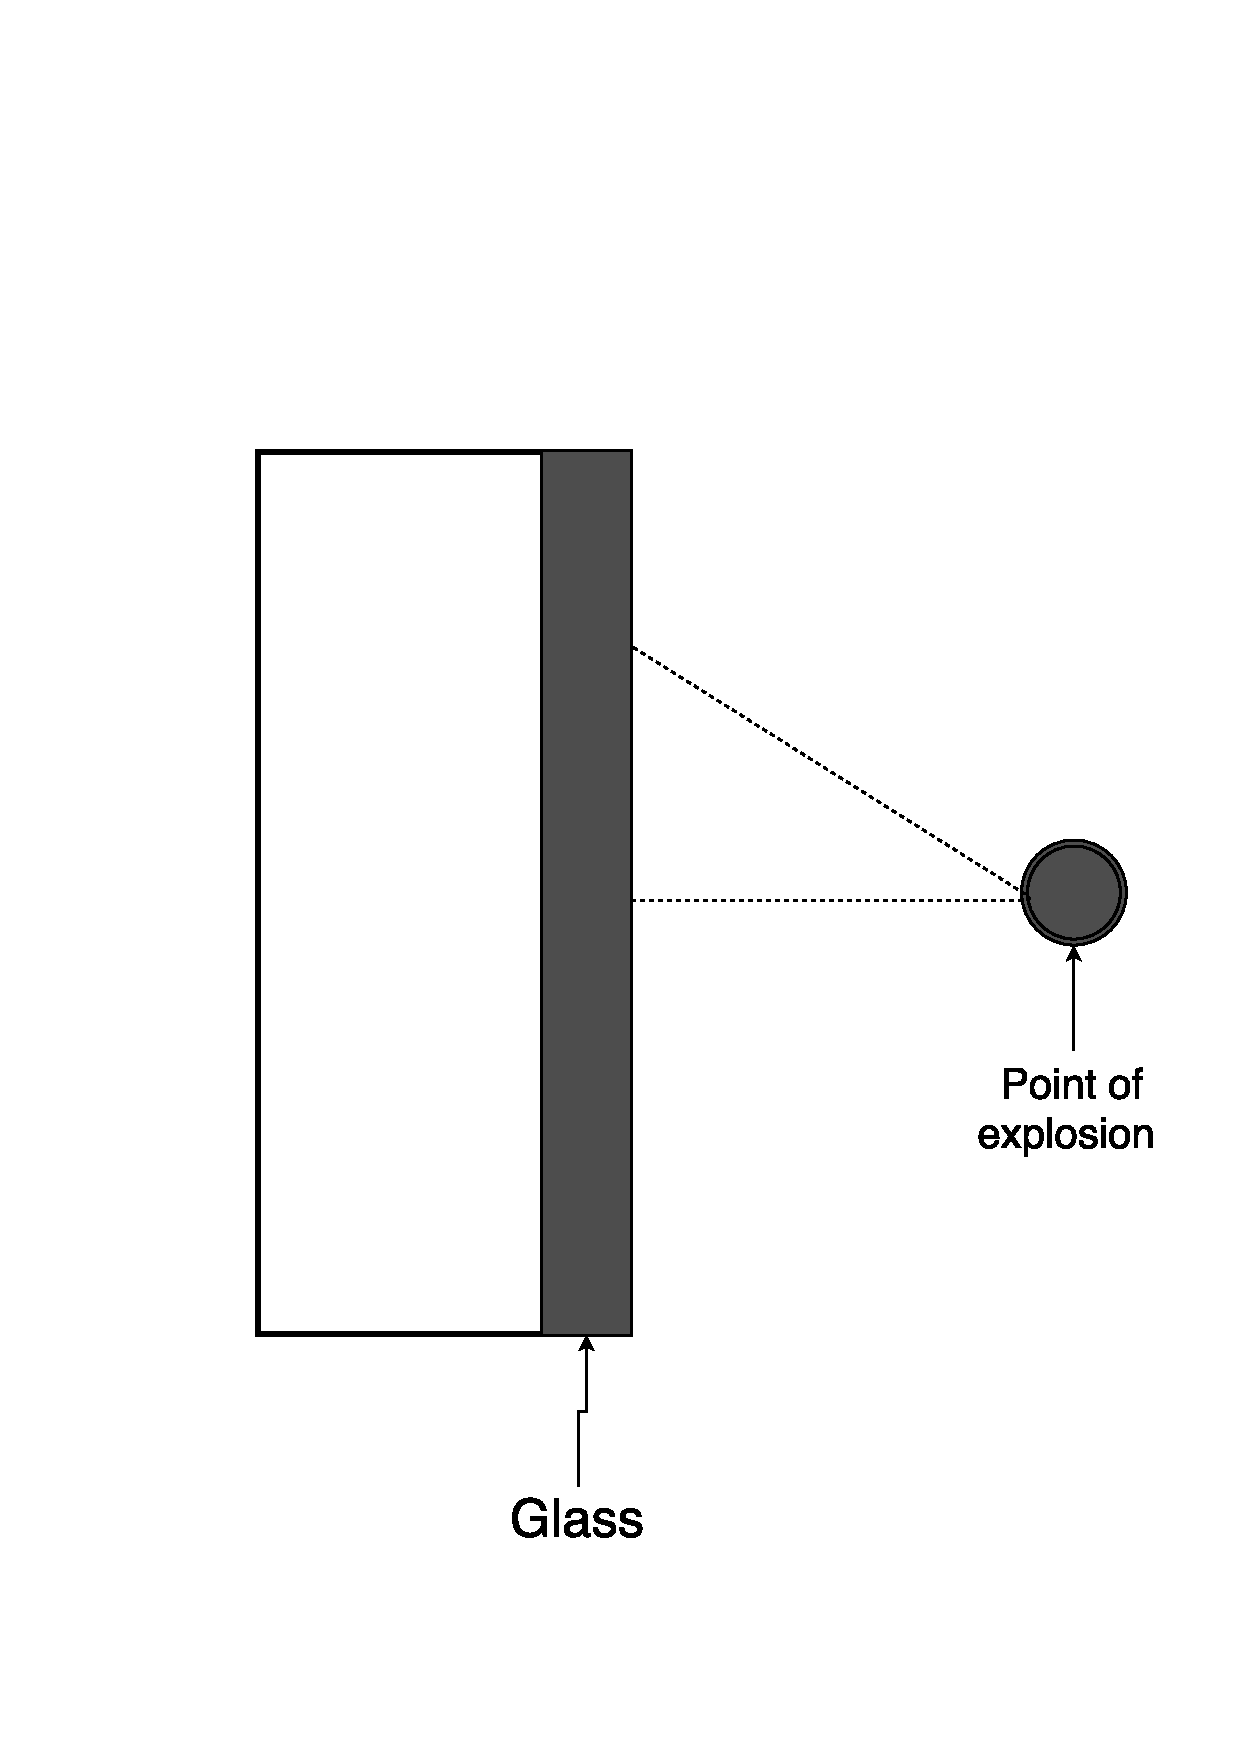
\includegraphics[scale=0.25]{physicalsystimage.pdf}
    \caption{The physical system}
    \label{Fig_PhysSyst}
  \end{center}
\end{figure}

\subsubsection{Goal Statements}

Given the dimensions of the glass plane, glass type, the characteristics of the explosion, and
the tolerable probability of breakage, the goal statements are:
\begin{itemize}
\item[GS\refstepcounter{goalnum}\thegoalnum:] Analyze and predict whether the
  glass slab under consideration will be able to withstand the explosion of a
  certain degree which is calculated based on user input.
\end{itemize}  

\subsection{Solution Characteristics Specification}

The instance models that govern \progname{} are presented in Section~\ref{sec_instmod}. The information
to understand the meaning of the instance models and their derivation is also presented, so
that the instance models can be verified.

\subsubsection{Assumptions} \label{Assumptions}

This section simplifies the original problem and helps in developing the
theoretical model by filling in the missing information for the physical
system. The numbers given in the square brackets refer to the Theoretical 
Models [Section~\ref{sec_theoretical}], General Definitions 
[Section~\ref{sec_gendef}], Data Definitions [Section~\ref{sec_datadef}], Instance
Models [Section~\ref{sec_instmod}], Likely Changes [Section~\ref{sec_like}],
or Unlikely Changes [Section~\ref{sec_unlike}], in which the respective 
assumption is used.

\begin{enumerate}

\item[A\refstepcounter{assumpnum}\theassumpnum \label{A_Glass}:] The standard E1300-09a for
  calculation applies only to monolithic, laminated, or insulating glass
  constructions of rectangular shape with continuous lateral support along one,
  two, three, or four edges.  This practice assumes that (1) the supported glass
  edges for two, three, and four-sided support conditions are simply supported
  and free to slip in plane; (2) glass supported on two sides acts as a simply
  supported beam and (3) glass supported on one side acts as a cantilever.

\item[A\refstepcounter{assumpnum}\theassumpnum \label{A_N/AGlass}:] Following \cite[(pg. 1)]{ASTM2009}, this practice does not apply to
  any form of wired, patterned, etched, sandblasted, drilled, notched, or grooved
  glass with surface and edge treatments that alter the glass strength.

\item [A\refstepcounter{assumpnum}\theassumpnum \label{A_External}:] This system
  only considers the external explosion scenario for its calculations.

\item[A\refstepcounter{assumpnum}\theassumpnum \label{ass_val}:] 
The values provided in Section~\ref{Sec:ValuofAuxiCons} are assumed for 
the duration of load ($t_d$), and the material properties of $m$, $k$, and $E$.  [\iref{IM_prob}, \ddref{DD_LDF}, 
\ddref{DD_NFL}, \ddref{DD_qhat}, \ddref{DD_JTOL}]

\item[A\refstepcounter{assumpnum}\theassumpnum \label{A_LSF}:] Glass under
  consideration is assumed to be a single lite; hence, the value of LSF is equal
  to 1 for all calculations in \progname.  [\iref{IM_cap}, \ddref{DD_qhat}]

\item[A\refstepcounter{assumpnum}\theassumpnum \label{A_BC}:] Boundary
  conditions for the glass slab are assumed to be 4-sided support for all
  calculations.  [\iref{IM_prob}]

 \item[A\refstepcounter{assumpnum}\theassumpnum \label{A_Flex}:] The response
   type considered in \progname{} is flexural.  [\iref{IM_prob}]

 \item[A\refstepcounter{assumpnum}\theassumpnum \label{A_LDF}:] With reference
   to A\ref{ass_val}, the value of load distribution factor (LDF) is a constant
   in \progname.  [\ddref{DD_LDF}]

\end{enumerate}

\subsubsection{Theoretical Models}\label{sec_theoretical}

This section focuses on the general equations and laws that \progname{} is based on.

~\newline
\noindent
\begin{minipage}{\textwidth}
\renewcommand*{\arraystretch}{1.5}
\begin{tabular}{| p{\colAwidth} | p{\colBwidth}|}
  \hline
  \rowcolor[gray]{0.9}
  Number& T\refstepcounter{theorynum}\thetheorynum \label{T_Pb}\\
  \hline
  Label&\bf Safety Req-Pb\\
  \hline
  Equation& $\text{is\_safe1}= P_b < P_{b_{\text{tol}}}$\\
  \hline
  Description 
  & If $\text{is\_safe1} = \text{True}$, the glass is considered safe.
    $\text{is\_safe1}$ and $\text{is\_safe2}$ (from \tref{T_LR}) are either both True or
    both False.\\
  & $P_b$ is the probability of breakage, as calculated in \iref{IM_prob}\\
  & $P_{b_{\text{tol}}}$ is the tolerable probability entered by the user\\
  \hline
  Source &
  \cite{ASTM2009}\\
  % The above web link should be replaced with a proper citation to a publication
  \hline
  Ref.\ By & \tref{T_LR}\\
  \hline
\end{tabular}
\end{minipage}\\

~\newline
\noindent
\begin{minipage}{\textwidth}
\renewcommand*{\arraystretch}{1.5}
\begin{tabular}{| p{\colAwidth} | p{\colBwidth}|}
  \hline
  \rowcolor[gray]{0.9}
  Number& T\refstepcounter{theorynum}\thetheorynum \label{T_LR}\\
  \hline
  Label &\bf Safety Req-LR\\
  \hline
  Equation & $\text{is\_safe2}= \text{LR} > q $\\
  \hline
  Description 
  & If $\text{is\_safe2} = \text{True}$, the glass is considered to be safe.
    $\text{is\_safe1}$ (from \tref{T_Pb}) and $\text{is\_safe2}$ are either both True or
    both False.\\
  & $\text{LR}$ is the Load Resistance (also called capacity), as defined in
    \iref{IM_cap}\\
  & $q$ (also referred as the demand) is the 3 second equivalent pressure, as
    defined in \iref{IM_dem}\\
  \hline
  Source &
           \cite{ASTM2009}\\
  % The above web link should be replaced with a proper citation to a publication
  \hline
  Ref.\ By & \tref{T_Pb}\\
  \hline
\end{tabular}
\end{minipage}\\
~\newline

\subsubsection{General Definitions}\label{sec_gendef}

There are no general definitions.


\subsubsection{Data Definitions}\label{sec_datadef}

This section collects and defines all the data needed to build the instance
models.

~\newline
\noindent
\begin{minipage}{\textwidth}
\renewcommand*{\arraystretch}{1.5}
\begin{tabular}{| p{\colAwidth} | p{\colBwidth}|}
  \hline
  \rowcolor[gray]{0.9}
  Number& DD\refstepcounter{datadefnum}\thedatadefnum \label{DD_B}\\
  \hline
  Label&\bf Risk of Failure (B)\\
  \hline
  Equation & $B = \frac{k}{(a \times b)^{m-1}}(E h^2)^m 
		  \times \text{LDF} \times e^J$\\
  \hline
  Description 
  & $B$ is the risk of failure\\
  & $m, k$ are the surface flaw parameters\\
  & $a$, $b$ are dimensions of the plate, where $(a>b)$\\
  & $E$ is the modulus of elasticity\\
  & $h$ is the true thickness, which is based on the nominal thickness as shown
    in \ddref{DD_thick}\\
  & $\text{LDF}$ is the Load Duration Factor, as defined in \ddref{DD_LDF}\\
  & $J$ is the stress distribution factor, as defined in \ddref{DD_J}\\  
  \hline
  Source &
  \cite{ASTM2009}, \cite[Eq.~14]{Campidelli}, \cite[Eq.~4-5]{BeasonEtAl1998}\\
  \hline
  Ref.\ By & \iref{IM_prob}\\
  \hline
\end{tabular}
\end{minipage}\\
~\newline

~\newline
\noindent
\begin{minipage}{\textwidth}
\renewcommand*{\arraystretch}{1.5}
\begin{tabular}{| p{\colAwidth} | p{\colBwidth}|}
  \hline
  \rowcolor[gray]{0.9}
  Number& DD\refstepcounter{datadefnum}\thedatadefnum \label{DD_thick}\\
  \hline
  Label&\bf Minimum Thickness ($h$)\\
  \hline
  Equation & $h = h(t)$\\
  \hline
  Description & 
  $h$ is a function that maps from the nominal thickness ($t$) to the minimum thickness, as follows:\\
  & $\begin{array}{rcrc}
h(t) \equiv ( t  = 2.5 \Rightarrow 2.16 & | & t = 2.7 \Rightarrow 2.59 & |\\
t = 3.0 \Rightarrow 2.92 & | & t = 4.0 \Rightarrow 3.78 & |\\
t = 5.0 \Rightarrow 4.57 & | & t = 6.0 \Rightarrow 5.56 & |\\
t = 8.0 \Rightarrow 7.42 & | & t = 10.0 \Rightarrow 9.02 & |\\
t = 12.0 \Rightarrow 11.91 & | & t = 16.0 \Rightarrow 15.09 & |\\
t = 19.0 \Rightarrow 18.26 & | & t = 22.0 \Rightarrow 21.44 & )\\
\end{array}$\\
  \hline
  Source &
  \cite{ASTM2009}\\
  \hline
  Ref.\ By & \iref{IM_prob}, \ddref{DD_JTOL}, \ddref{DD_qhat}, \ddref{DD_NFL}\\
  \hline
\end{tabular}
\end{minipage}\\
~\newline

~\newline
\noindent
\begin{minipage}{\textwidth}
\renewcommand*{\arraystretch}{1.5}
\begin{tabular}{| p{\colAwidth} | p{\colBwidth}|}
  \hline
  \rowcolor[gray]{0.9}
  Number& DD\refstepcounter{datadefnum}\thedatadefnum \label{DD_LDF}\\
  \hline
  Label&\bf Load Duration Factor (LDF)\\
  \hline
  Equation & $\text{LDF}=(\frac{t_d}{60})^{m/16}$\\
  \hline
  Description 
  & $t_d$ is the duration of the load\\
  & $m$ is a surface flaw parameter\\
  \hline
  Source &
  \cite{ASTM2009}\\
  % The above web link should be replaced with a proper citation to a publication
  \hline
  Ref.\ By & \iref{IM_prob}, \ddref{DD_JTOL}\\
  \hline
\end{tabular}
\end{minipage}\\

~\newline
~\newline
\noindent
\begin{minipage}{\textwidth}
\renewcommand*{\arraystretch}{1.5}
\begin{tabular}{| p{\colAwidth} | p{\colBwidth}|}
  \hline
  \rowcolor[gray]{0.9}
  Number& DD\refstepcounter{datadefnum}\thedatadefnum \label{DD_J}\\
  \hline
  Label&\bf Stress Distribution Factor $(J)$\\
  \hline
  Symbols & $J=J(\hat{q}, \mbox{AR})$ \\
  \hline
  Description  
        & $J$ is the stress distribution factor, which is obtained by
            interpolating from the data shown in Figure~\ref{ASTM_F2248-09_BeasonEtAl}\\
        & $\hat{q}$ is the dimensionless load defined in \ddref{DD_qhat}\\
        & AR is the aspect ratio defined in \ddref{DD_AR}\\
  \hline
  Source &
  \cite{ASTM2009}\\
  % The above web link should be replaced with a proper citation to a publication
  \hline
  Ref.\ By & \iref{IM_prob} \\
  \hline
\end{tabular}
\end{minipage}\\
~\newline

~\newline
\noindent
\begin{minipage}{\textwidth}
\renewcommand*{\arraystretch}{1.5}
\begin{tabular}{| p{\colAwidth} | p{\colBwidth}|}
  \hline
  \rowcolor[gray]{0.9}
  Number& DD\refstepcounter{datadefnum}\thedatadefnum \label{DD_NFL}\\
  \hline
  Label&\bf Non-Factored Load\\
  \hline
  Equations & $\text{NFL} = \frac{\hat{q}_{\text{tol}}Eh^4}{(ab)^2}$\\
  \hline
  Description 
  & $E$ is the modulus of elasticity\\
  & $a$, $b$ are the dimensions of the plate where $(a>b)$\\
  & $h$ is the true thickness, which is based on the nominal thickness as shown
    in \ddref{DD_thick}\\
  & $\hat{q}_{\text{tol}}$ is the tolerable load defined in \ddref{DD_qtol}\\
  \hline
  Source &
  \cite{ASTM2009}\\
  % The above web link should be replaced with a proper citation to a publication
  \hline
  Ref.\ By & \iref{IM_cap}\\
  \hline
\end{tabular}
\end{minipage}\\
~\newline

~\newline
\noindent
\begin{minipage}{\textwidth}
\renewcommand*{\arraystretch}{1.5}
\begin{tabular}{| p{\colAwidth} | p{\colBwidth}|}
  \hline
  \rowcolor[gray]{0.9}
  Number& DD\refstepcounter{datadefnum}\thedatadefnum \label{DD_GTF}\\
  \hline
  Label&\bf Glass Type Factor (GTF)\\
  \hline
  Equation & $\text{GTF} = \text{GTF}(g)$\\
  \hline
  Description & 
  $\text{GTF}$ is a function that maps from the glass type ($g$) to a real number, as follows:\\
  & $\text{GTF}(g) \equiv (g = \text{AN} \Rightarrow 1.0 | g = \text{FT}
    \Rightarrow 4.0 | g = \text{HS} \Rightarrow 2.0)$\\
  & AN is annealed glass\\
  & FT is fully tempered glass\\
  & HS is heat strengthened glass\\
  \hline
  Source &
  \cite{ASTM2009}\\
  % The above web link should be replaced with a proper citation to a publication
  \hline
  Ref.\ By & \ddref{DD_qhat}, \iref{IM_cap}\\
  \hline
\end{tabular}
\end{minipage}\\
~\newline

~\newline
\noindent
\begin{minipage}{\textwidth}
\renewcommand*{\arraystretch}{1.5}
\begin{tabular}{| p{\colAwidth} | p{\colBwidth}|}
  \hline
  \rowcolor[gray]{0.9}
  Number& DD\refstepcounter{datadefnum}\thedatadefnum \label{DD_qhat}\\
  \hline
  Label&\bf Dimensionless Load ($\hat{q}$)\\
  \hline
  Equation & $\hat{q}=\frac{q(ab)^2}{Eh^4 \text{GTF}}$\\
  \hline
  Description 
  & $q$ is the 3 second equivalent pressure, as given in \iref{IM_dem}\\
  & $a$, $b$ are dimensions of the plate, where $(a>b)$\\
  & $E$ is the modulus of elasticity \\
  & $h$ is the true thickness, which is based on the nominal thickness as shown
    in \ddref{DD_thick}\\
  & $\text{GTF}$ is the Glass Type Factor, as given by \ddref{DD_GTF}\\
  \hline
  Source &
  \cite{ASTM2009}, \cite[Eq.~7]{Campidelli}\\
  % The above web link should be replaced with a proper citation to a publication
  \hline
  Ref.\ By & \ddref{DD_J}\\
  \hline
\end{tabular}
\end{minipage}\\

~\newline

~\newline
\noindent
\begin{minipage}{\textwidth}
\renewcommand*{\arraystretch}{1.5}
\begin{tabular}{| p{\colAwidth} | p{\colBwidth}|}
  \hline
  \rowcolor[gray]{0.9}
  Number& DD\refstepcounter{datadefnum}\thedatadefnum \label{DD_qtol}\\
  \hline
  Label&\bf Tolerable Load ($\hat{q}_{\text{tol}}$)\\
  \hline
  Equations & $\hat{q}_{\text{tol}} = \hat{q}_{\text{tol}}(J_{\text{tol}}, \mbox{AR})$\\
  \hline
  Description 
        & $\hat{q}_{\text{tol}}$ is the tolerable load which is obtained from
          Figure~\ref{ASTM_F2248-09_BeasonEtAl} using $J_{\text{tol}}$ and Aspect Ratio
          $\mbox{AR}$ (\ddref{DD_AR}) as parameters using interpolation.  Calculation of $J_{\text{tol}}$
          is defined in \ddref{DD_JTOL}.\\
  \hline
  Source &
           \cite{ASTM2009}\\
  % The above web link should be replaced with a proper citation to a publication
  \hline
  Ref.\ By & \ddref{DD_NFL}\\
  \hline
\end{tabular}
\end{minipage}\\
~\newline

~\newline
\noindent
\begin{minipage}{\textwidth}
\renewcommand*{\arraystretch}{2}
\begin{tabular}{| p{\colAwidth} | p{\colBwidth}|}
  \hline
  \rowcolor[gray]{0.9}
  Number& DD\refstepcounter{datadefnum}\thedatadefnum \label{DD_JTOL}\\
  \hline
  Label&\bf Tolerable Stress Distribution Factor $(J_{\text{tol}})$\\
  \hline
  Symbols & $J_{\text{tol}}=\ln[\ln( \frac{1}{1-P_{b_{\text{tol}}}} )
				\frac{(a \times b)^{m-1}}
				{k(E h^2)^m \text{LDF} }]$ \\  
  \hline
  Description  &
  $J_{\text{tol}}$ is the stress distribution factor calculated with reference to $P_{b_{\text{tol}}}$\\
  & $a$, $b$ are dimensions of the plate where $(a>b)$\\
  & $h$ is the true thickness, which is based on the nominal thickness as shown
    in \ddref{DD_thick}\\
  & $m$, $k$ are the surface flaw parameters\\
  & $\text{LDF}$ is the Load Duration Factor, as defined by \ddref{DD_LDF}\\
  & $E$ is the modulus of elasticity\\ 
  & $P_{b_{\text{tol}}}$ is the tolerable probability entered by the user\\  
  \hline
  Source &
  \cite{ASTM2009}\\
  % The above web link should be replaced with a proper citation to a publication
  \hline
  Ref.\ By & \ddref{DD_qtol} \\
  \hline
\end{tabular}
\end{minipage}\\
~\newline

~\newline
\noindent
\begin{minipage}{\textwidth}
\renewcommand*{\arraystretch}{1.5}
\begin{tabular}{| p{\colAwidth} | p{\colBwidth}|}
  \hline
  \rowcolor[gray]{0.9}
  Number& DD\refstepcounter{datadefnum}\thedatadefnum \label{DD_SD}\\
  \hline
  Label&\bf Stand off Distance (SD)\\
  \hline
  Equations & $\mbox{SD} = \sqrt{{\text{SD}_x}^2 + {\text{SD}_y}^2 + {\text{SD}_z}^2}$\\
  \hline
  Description 
  & $\text{SD}$ is the stand off distance and
    $(\text{SD}_x,\text{SD}_y,\text{SD}_z)$ are the coordinates for this position\\
  \hline
  Source &
  \cite{ASTM2009}\\
  \hline
  Ref.\ By & \iref{IM_dem}\\
  \hline
\end{tabular}
\end{minipage}\\
~\newline

~\newline
\noindent
\begin{minipage}{\textwidth}
\renewcommand*{\arraystretch}{1.5}
\begin{tabular}{| p{\colAwidth} | p{\colBwidth}|}
  \hline
  \rowcolor[gray]{0.9}
  Number& DD\refstepcounter{datadefnum}\thedatadefnum \label{DD_AR}\\
  \hline
  Label&\bf Aspect Ratio (AR)\\
  \hline
  Equations & $\mbox{AR} = a/b$\\
  \hline
  Description 
  & $\text{AR}$ is the Aspect Ratio and $a$, $b$ are dimensions of the plate
    where $(a \geq b)$\\
  \hline
  Source &
  \cite{ASTM2009}\\
  \hline
  Ref.\ By & \ddref{DD_J}, \ddref{DD_qtol}\\
  \hline
\end{tabular}
\end{minipage}\\
~\newline

\subsubsection{Instance Models}\label{sec_instmod}
This section transforms the problem defined in Section~\ref{sec_probdesc} into one 
which is expressed in mathematical terms. It uses concrete symbols defined in Section~\ref{sec_datadef} 
to replace the abstract symbols in the models identified in Section~\ref{sec_theoretical} 
and Section~\ref{sec_gendef}.

\noindent
\begin{minipage}{\textwidth}
\renewcommand*{\arraystretch}{1.5}
\begin{tabular}{| p{\colAwidth} | p{\colBwidth}|}
  \hline
  \rowcolor[gray]{0.9}
  Number& IM\refstepcounter{instnum}\theinstnum \label{IM_prob} \\
  \hline
  Label&\bf Probability of Glass Breakage\\
  \hline
  Equation& $P_b = 1-e^{-B}$\\
\hline
  Description & $P_b$ is the calculated probability of breakage\\
  & $B$ is the risk of failure, as defined in \ddref{DD_B}\\
  \hline
  Source &
  \cite{ASTM2009, BeasonEtAl1998}\\
  \hline
  Ref.\ By & \tref{T_Pb}\\
  \hline
\end{tabular}
\end{minipage}\\
~\newline

\noindent
\begin{minipage}{\textwidth}
\renewcommand*{\arraystretch}{1.5}
\begin{tabular}{| p{\colAwidth} | p{\colBwidth}|}
  \hline
  \rowcolor[gray]{0.9}
  Number& IM\refstepcounter{instnum}\theinstnum \label{IM_cap} \\
  \hline
  Label&\bf Calculation of Capacity (LR)\\
  \hline
  Equation& $\text{LR} = \text{NFL} \times \text{GTF} \times \text{LSF}$\\ 
\hline
  Description 
  & $\text{LR}$ is the Load Resistance, which is also called capacity\\
  & $\text{NFL}$ is the Non-Factored Load, as defined in \ddref{DD_NFL}\\
  &$\text{GTF}$ is the Glass Type Factor, as given by \ddref{DD_GTF}\\
  & $\text{LSF}$ is the Load Share Factor\\
  \hline
  Source &
           \cite{ASTM2009}\\
  \hline
  Ref.\ By & \tref{T_LR}\\
  \hline
\end{tabular}
\end{minipage}\\

~\newline
\noindent
\begin{minipage}{\textwidth}
\renewcommand*{\arraystretch}{1.5}
\begin{tabular}{| p{\colAwidth} | p{\colBwidth}|}
  \hline
  \rowcolor[gray]{0.9}
  Number& IM\refstepcounter{instnum}\theinstnum \label{IM_dem} \\
  \hline
  Label&\bf Calculation of Demand ($q$)\\
  \hline
  Equation& $q=q(w_{\text{TNT}}, \text{SD}$)\\ 
\hline
  Description & $q$, or demand, is the 3 second equivalent pressure obtained from the
                Figure~\ref{Fig_ASTM_F2248-09} by interpolation using stand off distance $(\text{SD})$ and
                $w_{\text{TNT}}$ as parameters\\
  & $w_{\text{TNT}}$ is defined as $w_{\text{TNT}}= w \times \text{TNT} $\\
   &$w$ is the charge weight\\
  & $\text{TNT}$ is the TNT equivalent factor\\
  & $\text{SD}$ is the stand off distance (\ddref{DD_SD})\\
  \hline
  Source &
  \cite{ASTM2009}\\
  \hline
  Ref.\ By & \tref{T_LR}, \ddref{DD_qhat}\\
  \hline
\end{tabular}
\end{minipage}\\

\subsubsection{Data Constraints} \label{sec_DataConstraints}

Table~\ref{TblInputVar} and Table~\ref{TblOutputVar} show the data constraints on the input and output variables, respectively.  The
column of physical constraints gives the physical limitations on the range of
values that can be taken by the variable. The uncertainty column (``Uncert." stands for ``Uncertainty") provides an estimate of the confidence
with which the physical quantities can be measured.  This information would be
part of the input if one were performing an uncertainty quantification exercise. The constraints are conservative, to
give the user of the model the flexibility to experiment with unusual
situations.  The column of typical values is intended to provide a feel for a
common scenario.
Section~\ref{Sec:ValuofAuxiCons} gives the values of the specification parameters used
in Table~\ref{TblInputVar}.

\begin{table}[!h]
\caption{Input Variables} \label{TblInputVar}
\renewcommand{\arraystretch}{1.2}
\begin{tabular}{l l l l c} 
\toprule
\textbf{Var} & \textbf{Physical Constraints} & \textbf{Software Constraints} & \textbf{Typical Value} & \textbf{Uncert.} \\
\midrule 
$a$&$a > 0 \wedge \text{AR} \geq 1$ & $d_{\text{min}} \leq a \leq d_{\text{max}} \wedge \text{AR}
                           < \text{AR}_{\text{max}}$ & 1.5 \si[per-mode=symbol] {\metre}& 10\%\\
                           
$b$&$0 < b \leq a$ & $d_{\text{min}} \leq b \leq d_{\text{max}} \wedge \text{AR}
                           < \text{AR}_{\text{max}}$ & 1.2 \si[per-mode=symbol]{\metre}& 10\%\\
                           
$P_{b_{\text{tol}}}$& $0 < P_{b_{\text{tol}}} < 1$& --& 0.008 &0.1\%\\

$\text{SD}$&$\text{SD}>0$&$\text{SD}_{\text{min}}<\text{SD}<\text{SD}_{\text{max}}$&45
\si[per-mode=symbol]{\meter}&10\%\\

$\text{TNT}$&$\text{TNT}>0$&--&1.0&10\%\\

%$t$&$t>0$&--&6\si[per-mode=symbol] {\milli\metre}&10\%\\

$w$&$w > 0$ & $w_{\text{min}} \le w \le w_{\text{max}}$&42 \si[per-mode=symbol]{\kilo\gram}&10\%\\

\bottomrule
\end{tabular}
\end{table}

Note: The values for $d_\text{min}$ and $d_\text{max}$ are obtained from Figure~\ref{Fig_ASTM_E1300-09}
and the GLASS\textunderscore BR\textunderscore 0\textunderscore 40b.xslm which can be found in the 
Reference directory. The value for $\mbox{AR}_\text{max}$ is obtained from Figure~\ref{ASTM_F2248-09_BeasonEtAl}
and the GLASS\textunderscore BR\textunderscore 0\textunderscore 40b.xslm.
The values for $w_\text{min}$, $w_\text{max}$, $\text{SD}_\text{min}$ and $\text{SD}_\text{max}$
are obtained from Figure~\ref{Fig_ASTM_F2248-09} and the GLASS\textunderscore BR\textunderscore 0\textunderscore 40b.xslm. 
\newline

\begin{figure}[h!]
  \begin{center}
    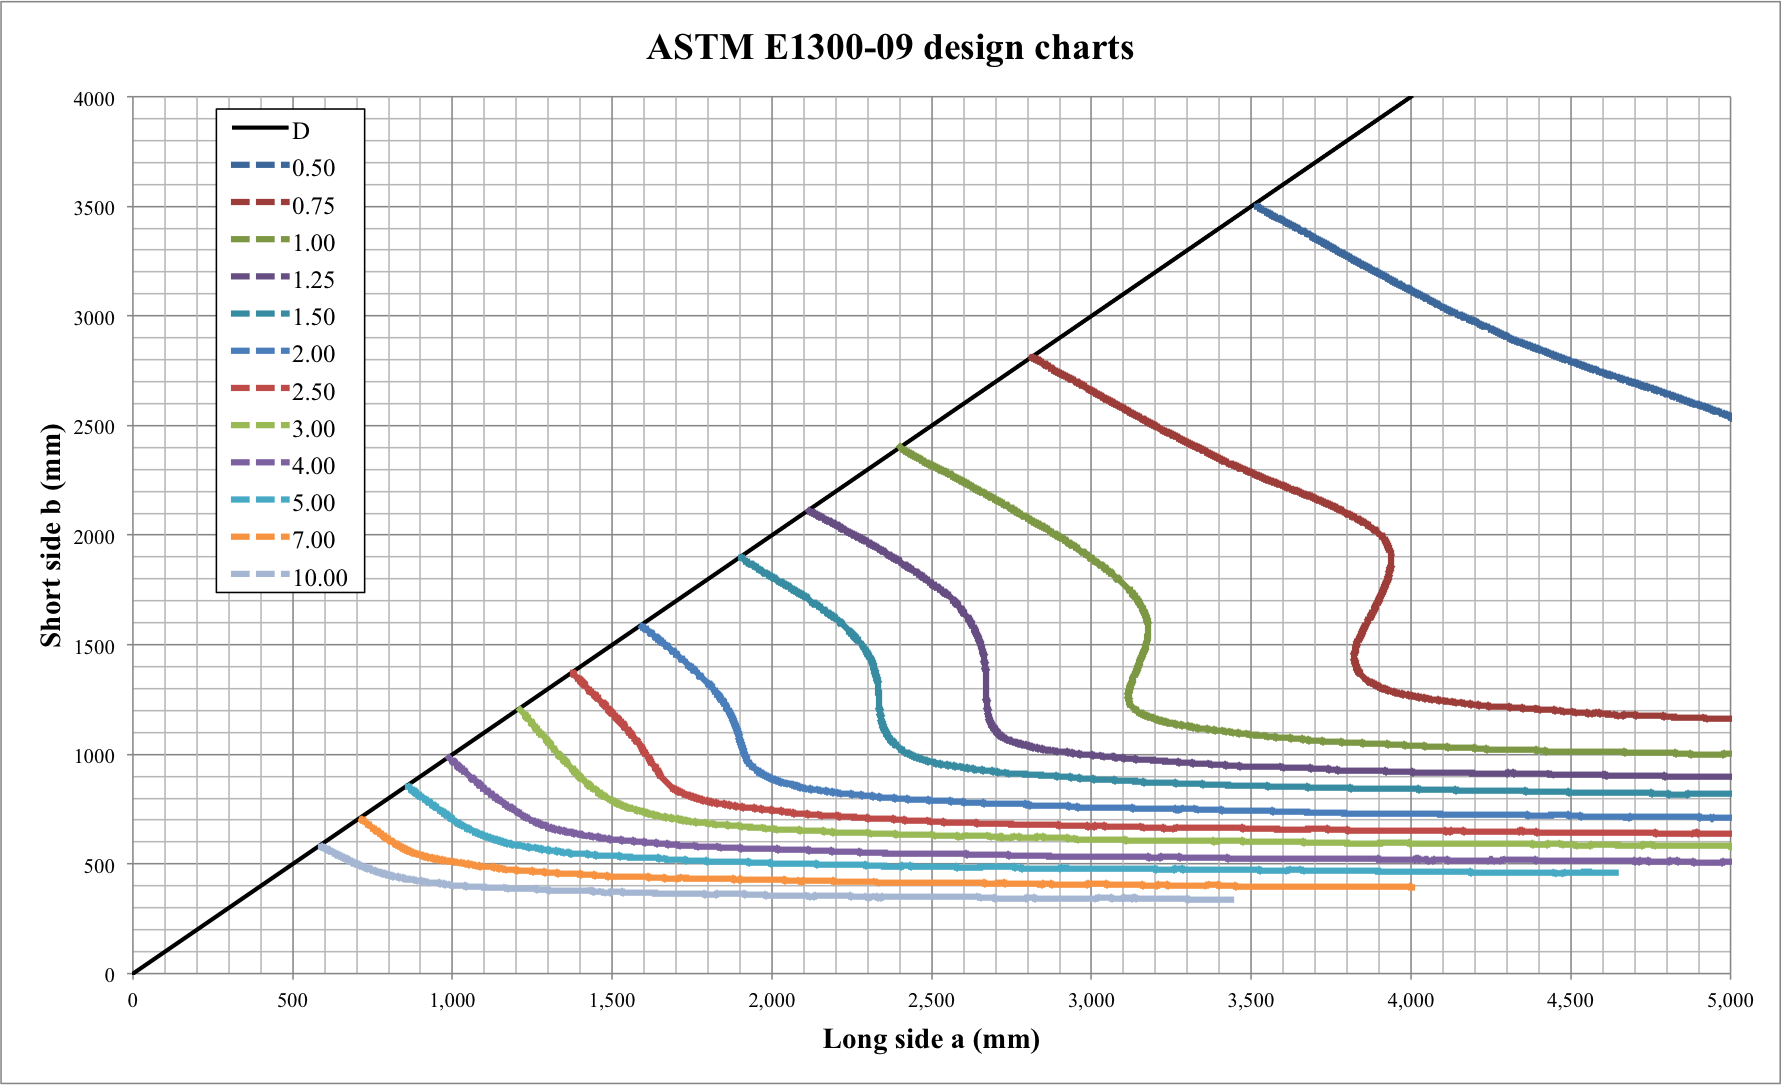
\includegraphics[width=\textwidth]{ASTM_E1300-09_design_charts.png}
    \caption{Long side (a) versus Short side (b)}
    \label{Fig_ASTM_E1300-09}
  \end{center}
\end{figure}

\begin{table}[!h]
\caption{Output Variables} \label{TblOutputVar}
\renewcommand{\arraystretch}{1.2}
\begin{center}
\begin{tabular}{l c} 
\toprule
\textbf{Var} & \textbf{Physical Constraints} \\
\midrule 
$P_b$ & $0 < P_b < 1$\\
\bottomrule
\end{tabular}
\end{center}
\end{table}
  
\section{Requirements}  
  
\subsection{Functional Requirements} \label{Func}

The following section provides the functional requirements, the business tasks
that the software is expected to complete.

\noindent \begin{itemize}

\item[R\refstepcounter{reqnum}\thereqnum \label{Input}:] Input the following
  quantities, which define the glass dimensions, type of glass, tolerable probability of
  failure and the characteristics of the blast:

\renewcommand{\arraystretch}{1.2}
\begin{tabular}{l l p{11cm}} 
\toprule
\textbf{symbol} & \textbf{unit} & \textbf{description}\\
\midrule 
$a$ & \si{\metre}	& Length of the glass slab\\
$b$ & \si{\metre}	& Breadth of the glass slab\\
$g$ & -- & Glass Type, $g \in \{ \text{AN}, \text{HS}, \text{GT} \}$\\
$P_{b_{\text{tol}}}$ & -- & Tolerable probability\\
$\text{SD}_x$ & \si{\meter} & Stand off distance ($x$-component)\\
$\text{SD}_y$ & \si{\metre} & Stand off distance ($y$-component)\\
$\text{SD}_z$ & \si{\metre} & Stand off distance ($z$-component)\\
$t$ & \si{\milli\metre}	& Nominal thickness of the glass slab,\newline $t \in
                                  \{2.5, 2.7, 3.0, 4.0, 5.0, 6.0, 8.0, 10.0,
                                  12.0, 16.0, 19.0, 22.0\}$ \\
$\text{TNT}$ & -- & TNT equivalent factor\\
$w$ & \si{\kilo\gram}	& Charge weight\\
\bottomrule
\end{tabular}

\item [R\refstepcounter{reqnum}\thereqnum \label{KnownValues}:]

The system shall set the known values as follows:
\begin{itemize}
\item $m$, $k$, $E$, $t_d$ following \aref{ass_val}
\item LDF from \ddref{DD_LDF}
\item LSF following \aref{A_LSF}
\item $h$ from \ddref{DD_thick}
\item GTF from \ddref{DD_GTF}
\item SD from \ddref{DD_SD}
\item AR from \ddref{DD_AR}
\end{itemize}

\item[R\refstepcounter{reqnum}\thereqnum \label{Verify}:]

  The system shall check the entered input values to ensure that they do not
  exceed the data constraints mentioned in \ref{sec_DataConstraints}.  If any of
  the input parameters is out of bounds, an error message is displayed and the
  calculations stop.

\item[R\refstepcounter{reqnum}\thereqnum \label{R_OutputInput}:]

  Output the input quantities from~\rref{Input} and the known quantities
  from~\rref{KnownValues}.

% \item[R\refstepcounter{reqnum}\thereqnum \label{R_Interpolation}:]
%   Some of the values requires for calculations are present in form of
%   graphs. Hence the system is expected to do linear interpolation to extract
%   values of a certain parameter from the graphs. \\

\item[R\refstepcounter{reqnum}\thereqnum \label{R_ Comparison}:] If
  $\text{is\_safe1} \wedge \text{is\_safe2}$ (from \tref{T_Pb} and \tref{T_LR}) are true,
  output the message ``For the given input parameters, the glass is considered
  safe.''  If the condition is false, then output the message ``For the given
  input parameters, the glass is NOT considered safe.''

\item[R\refstepcounter{reqnum}\thereqnum \label{R_Output}:]
  Output the following quantities:
\begin{itemize}
\item Probability of breakage ($P_b$) (\iref{IM_prob})
\item Risk of failure ($B$) (\ddref{DD_B})
\item Load resistance (LR) (\iref{IM_cap})
\item Applied load (demand) ($q$) (\iref{IM_dem})
\item Stress distribution factor ($J$) (\ddref{DD_J})
\item Non-factored load (NFL) (\ddref{DD_NFL})
\item Glass type factor (GTF) (\ddref{DD_GTF})
\item Dimensionless load ($\hat{q}$) (\ddref{DD_qhat})
\item Tolerable load ($\hat{q}_{\text{tol}}$) (\ddref{DD_qtol})
\item Stress distribution factor based on $P_b$ ($J_{\text{tol}}$) (\ddref{DD_JTOL})
\item Minimum thickness ($h$) (\ddref{DD_thick})
\item Aspect Ratio (AR) (\ddref{DD_AR})
\end{itemize}

\end{itemize}

\subsection{Nonfunctional Requirements}

Given the small size, and relative simplicity, of this problem, performance is
not a priority.  Any reasonable implementation will be very quick and use
minimal storage.  Rather than performance, the priority nonfunctional
requirements are correctness, verifiability, understandability, reusability, 
maintainability and portability.

\section{Likely Changes} \label{sec_like}

\noindent \begin{itemize}

\item[LC\refstepcounter{lcnum}\thelcnum\label{LC_int}:] \aref{A_External} - The
  system currently only calculates for external blast risk. In the future,
  calculations can be added for the internal blast risk.

% \item[LC\refstepcounter{lcnum}\thelcnum\label{new}:] As new information becomes
%   relevant different methods might be used to analyze and interpret the
%   inputs.

\item[LC\refstepcounter{lcnum}\thelcnum\label{LC_variables}:] \aref{ass_val},
  \aref{A_LDF} - Currently, the values for $m$, $k$ and $E$ are assumed to be the
  same for all glass.  In the future, these values can be changed to variable
  inputs.

\item[LC\refstepcounter{lcnum}\thelcnum\label{LC_lite}:] \aref{A_LSF} - The
  software may be changed to accommodate more than a single lite.

\item[LC\refstepcounter{lcnum}\thelcnum\label{LC_BC}:] \aref{A_BC} - The
  software may be changed to accommodate more boundary conditions than 4-sided
  support.

\item[LC\refstepcounter{lcnum}\thelcnum\label{LC_Flex}:] \aref{A_Flex} - The
  software may be changed to consider more than just flexure of the glass.

% \item[LC\refstepcounter{lcnum}\thelcnum\label{LC_output}:] The interface of the
%   system can be changed according e with respect to the client wishes in the
%   future.

\end{itemize}

\section{Unlikely Changes} \label{sec_unlike}

\noindent \begin{itemize}

\item[\refstepcounter{ucnum} \utheucnum \label{ucGoal}:] The goal of the system
  is to predict whether the glass slab under consideration can withstand an 
  explosion of a certain degree.
\item[\refstepcounter{ucnum} \utheucnum \label{ucN/AGlass}:] \aref{A_N/AGlass} requires that the glass is not altered in any way. Therefore, this cannot be used on altered glass.

\end{itemize}

\section{Traceability Matrices and Graphs}
The purpose of the traceability matrices is to provide easy references on what 
has to be additionally modified if a certain component is changed.  Every time a 
component is changed, the items in the column of that component that are 
marked with an ``X'' should be modified as well.  Table~\ref{Table:trace}
shows the dependencies of theoretical models, instance models, and data 
definitions with each other. Table~\ref{Table:R_trace} shows the dependencies of 
requirements on theoretical models, instance models, data definitions and 
data constraints. Table~\ref{Table:A_trace} shows the dependencies 
of theoretical models, instance models, data definitions, likely changes and 
requirements on the assumptions.
\newline

\begin{table}[h!]
\centering
\begin{tabular}{|c|c|c|c|c|c|c|c|c|c|c|c|c|c|c|}
\hline        
	& \tref{T_Pb} & \tref{T_LR} & \iref{IM_prob} & \iref{IM_cap}& \iref{IM_dem} & 
	\ddref{DD_B} & \ddref{DD_thick} & \ddref{DD_LDF} & \ddref{DD_J} & \ddref{DD_NFL} & 
	\ddref{DD_GTF} & \ddref{DD_qhat} & \ddref{DD_qtol} & \ddref{DD_JTOL} \\
\hline
\tref{T_Pb}           & & X & X & & & & & & & & & & & \\ \hline
\tref{T_LR}             & X & & & X & X & & & & & & & & & \\ \hline
\iref{IM_prob}      & & & & & & X & X & X & X & & & & & \\ \hline
\iref{IM_cap}        & & & & & & & & & & X & X & & & \\ \hline
\iref{IM_dem}       & & & & & & & & & & & & & & \\ \hline
\ddref{DD_B}       & & & & & & & & & & & & & & \\ \hline
\ddref{DD_thick}  & & & & & & & & & & & & & & \\ \hline
\ddref{DD_LDF}   & & & & & & & & & & & & & & \\ \hline
\ddref{DD_J}        & & & & & & & & & & & & X & & \\ \hline
\ddref{DD_NFL}   & & & & & & & X & & & & & & X & \\ \hline
\ddref{DD_GTF}   & & & & & & & & & & & & & & \\ \hline
\ddref{DD_qhat}   & & & & & X & & X & & & & X & & & \\ \hline
\ddref{DD_qtol}    & & & & & & & & & & & & & & X \\ \hline
\ddref{DD_JTOL} & & & & & & & X & X & & & & & & \\
\hline
\end{tabular}
\caption{Traceability Matrix Showing the Connections Between Items of Different Sections}
\label{Table:trace}
\end{table}

\newpage

\begin{table}[h!]
\centering
\begin{tabular}{|P{0.4cm}|P{0.4cm}|P{0.4cm}|P{0.6cm}|P{0.6cm}|P{0.6cm}|P{0.65cm}|
P{0.65cm}|P{0.65cm}|P{0.65cm}|P{0.65cm}|P{0.65cm}|P{0.65cm}|P{0.65cm}|P{0.65cm}|
P{0.8cm}|P{0.4cm}|P{0.4cm}|}
\hline
	& \tref{T_Pb} & \tref{T_LR} & \iref{IM_prob} & \iref{IM_cap} &
	\iref{IM_dem} & \ddref{DD_B} & \ddref{DD_thick} & \ddref{DD_LDF} &
	\ddref{DD_J} & \ddref{DD_NFL} & \ddref{DD_GTF} & \ddref{DD_qhat} &
	\ddref{DD_qtol} & \ddref{DD_JTOL} & \ref{sec_DataConstraints} &
	\rref{Input} & \rref{KnownValues}\\
\hline
\rref{Input}                 & & & & & & & & & & & & & & & & & \\ \hline
\rref{KnownValues}   & & & & & & & & & & & & & & & & & \\ \hline
\rref{Verify}                & & & & & & & & & & & & & & & X & & \\ \hline
\rref{R_OutputInput}  & & & & & & & & & & & & & & & & X & X \\ \hline
\rref{R_ Comparison}  & X & X & & & & & & & & & & & & & & & \\ \hline
\rref{R_Output}          & & & X & X & X & & X & X & X & X & X & X & X & X & & & \\
\hline
\end{tabular}
\caption{Traceability Matrix Showing the Connections Between Requirements and Other Items.}
\label{Table:R_trace}
\end{table}

\newpage

\begin{table}[h!]
\centering
\begin{tabular}{|c|c|c|c|c|c|c|c|c|c|}
\hline
	& \aref{A_Glass}& \aref{A_N/AGlass}& \aref{A_External}& \aref{ass_val}& 
	\aref{A_LSF}& \aref{A_BC}& \aref{A_Flex}& \aref{A_LDF}\\
\hline
\tref{T_Pb}                 & & & & & & & & \\ \hline
\tref{T_LR}                  & & & & & & & & \\ \hline
\iref{IM_prob}           & & & & X & & X & X & \\ \hline
\iref{IM_cap}             & & & & & X & & & \\ \hline
\iref{IM_dem}            & & & & & & & & \\ \hline
\ddref{DD_B}            & & & & & & & & \\ \hline
\ddref{DD_thick}       & & & & & & & & \\ \hline
\ddref{DD_LDF}        & & & & X & & & & X \\ \hline
\ddref{DD_J}             & & & & & & & & \\ \hline
\ddref{DD_NFL}        & & & & X & & & & \\ \hline
\ddref{DD_GTF}        & & & & & & & & \\ \hline
\ddref{DD_qhat}        & & & & & X & & & \\ \hline
\ddref{DD_qtol}         & & & & & & & & \\ \hline
\ddref{DD_JTOL}      & & & & X & & & & \\ \hline
\lcref{LC_int}             & & & X & & & & & \\ \hline
\lcref{LC_variables}   & & & & X & & & & X \\ \hline
\lcref{LC_lite}             & & & & & X & & & \\ \hline
\lcref{LC_BC}             & & & & & & X & & \\ \hline
\lcref{LC_Flex}           & & & & & & & X &\\ \hline
\rref{Input}                  & & & & & & & & \\ \hline
\rref{KnownValues}     & & & & X & X & & & X \\ \hline
\rref{Verify}                 & & & & & & & & \\ \hline
\rref{R_OutputInput}   & & & & & & & & \\ \hline
\rref{R_ Comparison} & & & & & & & & \\ \hline
\rref{R_Output}           & & & & & & & & \\
\hline
\end{tabular}
\caption{Traceability Matrix Showing the Connections Between Assumptions and Other Items}
\label{Table:A_trace}
\end{table}

\newpage

The purpose of the traceability graphs is also to provide easy references 
on what has to be additionally modified if a certain component is changed.  
The arrows in the graphs represent dependencies. The component at the 
tail of an arrow is depended on by the component at the head of that arrow. 
Therefore, if a component is changed, the components that it points to should 
also be changed. Figure~\ref{Fig_Trace} shows the dependencies of 
theoretical models, instance models, and data definitions on each other. 
Figure~\ref{Fig_RTrace} shows the dependencies of requirements on 
theoretical models, instance models, data definitions and data constraints.
Figure~\ref{Fig_ATrace} shows the dependencies of theoretical models,
instance models, data definitions, requirements and likely changes on assumptions.
 
NOTE: Building a tool to automatically generate the graphical 
representation of the matrix by scanning the labels and reference can be 
future work.

\begin{figure}[h!]
	\begin{center}
		%\rotatebox{-90}
		{
			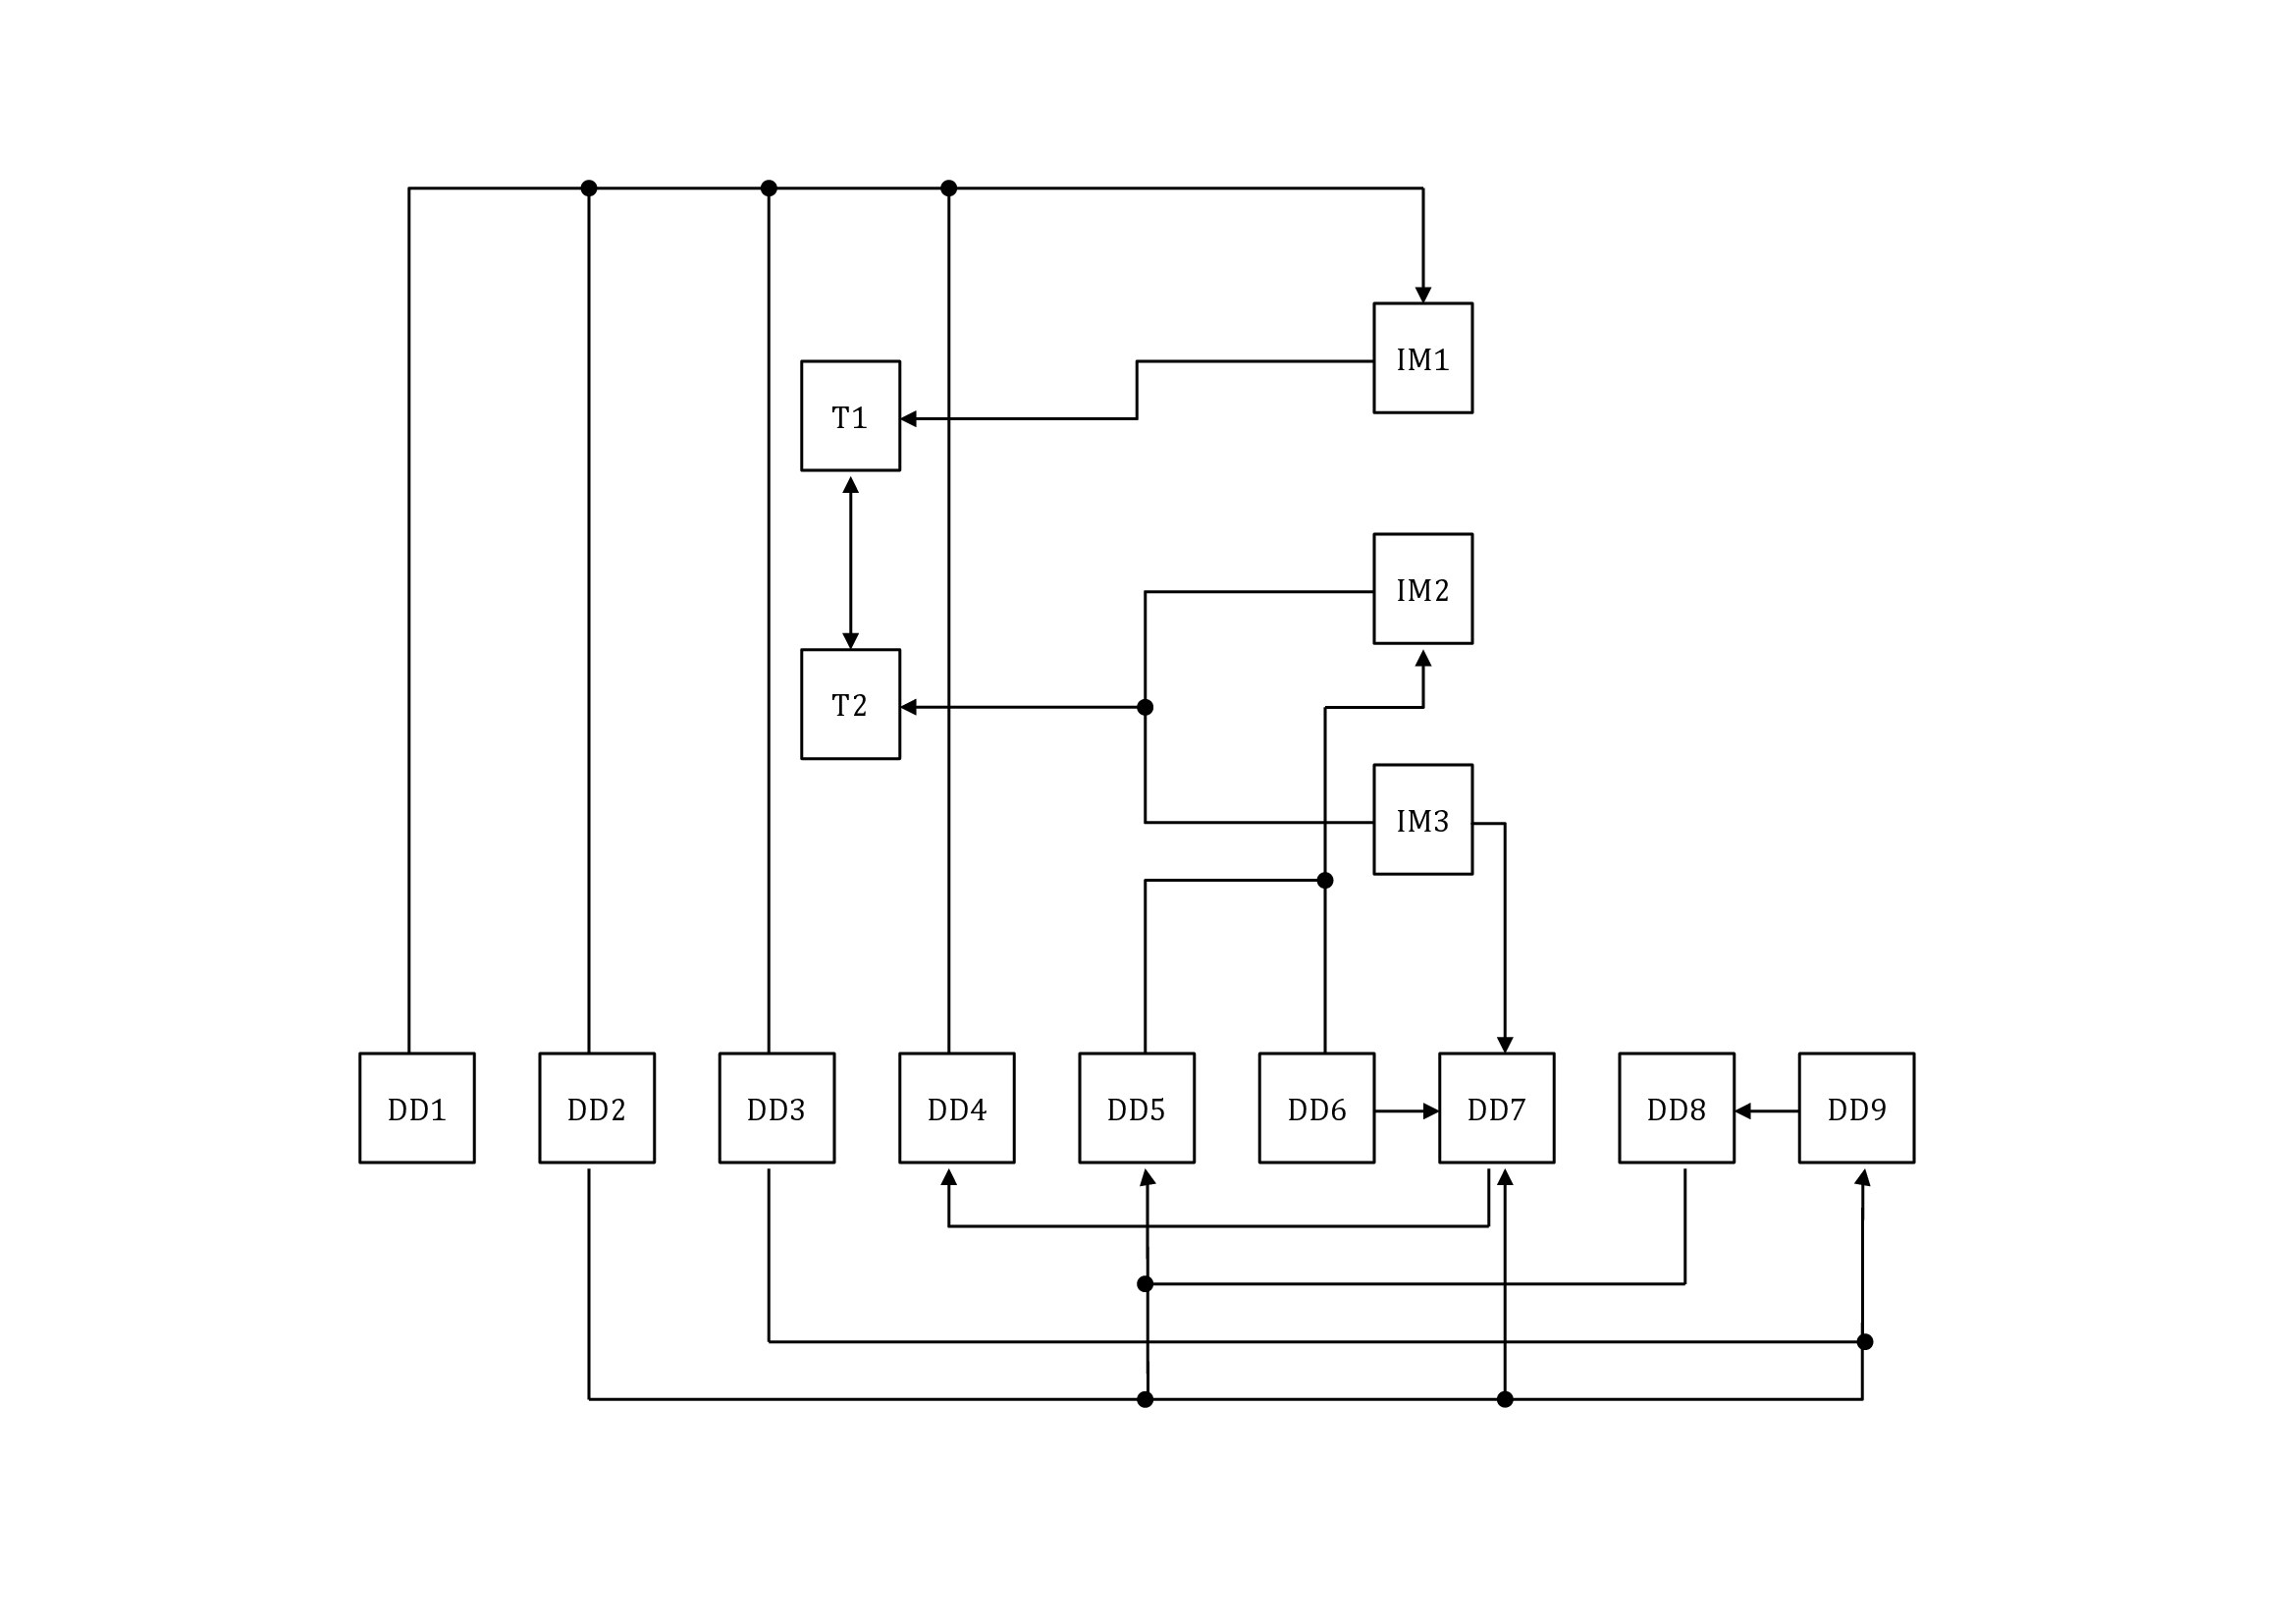
\includegraphics[width=\textwidth]{Trace.png}
		}
		\caption{\label{Fig_Trace} Traceability Graph Showing the Connections Between Items of Different Sections.}
	\end{center}
\end{figure}

\begin{figure}[h!]
	\begin{center}
		%\rotatebox{-90}
		{
			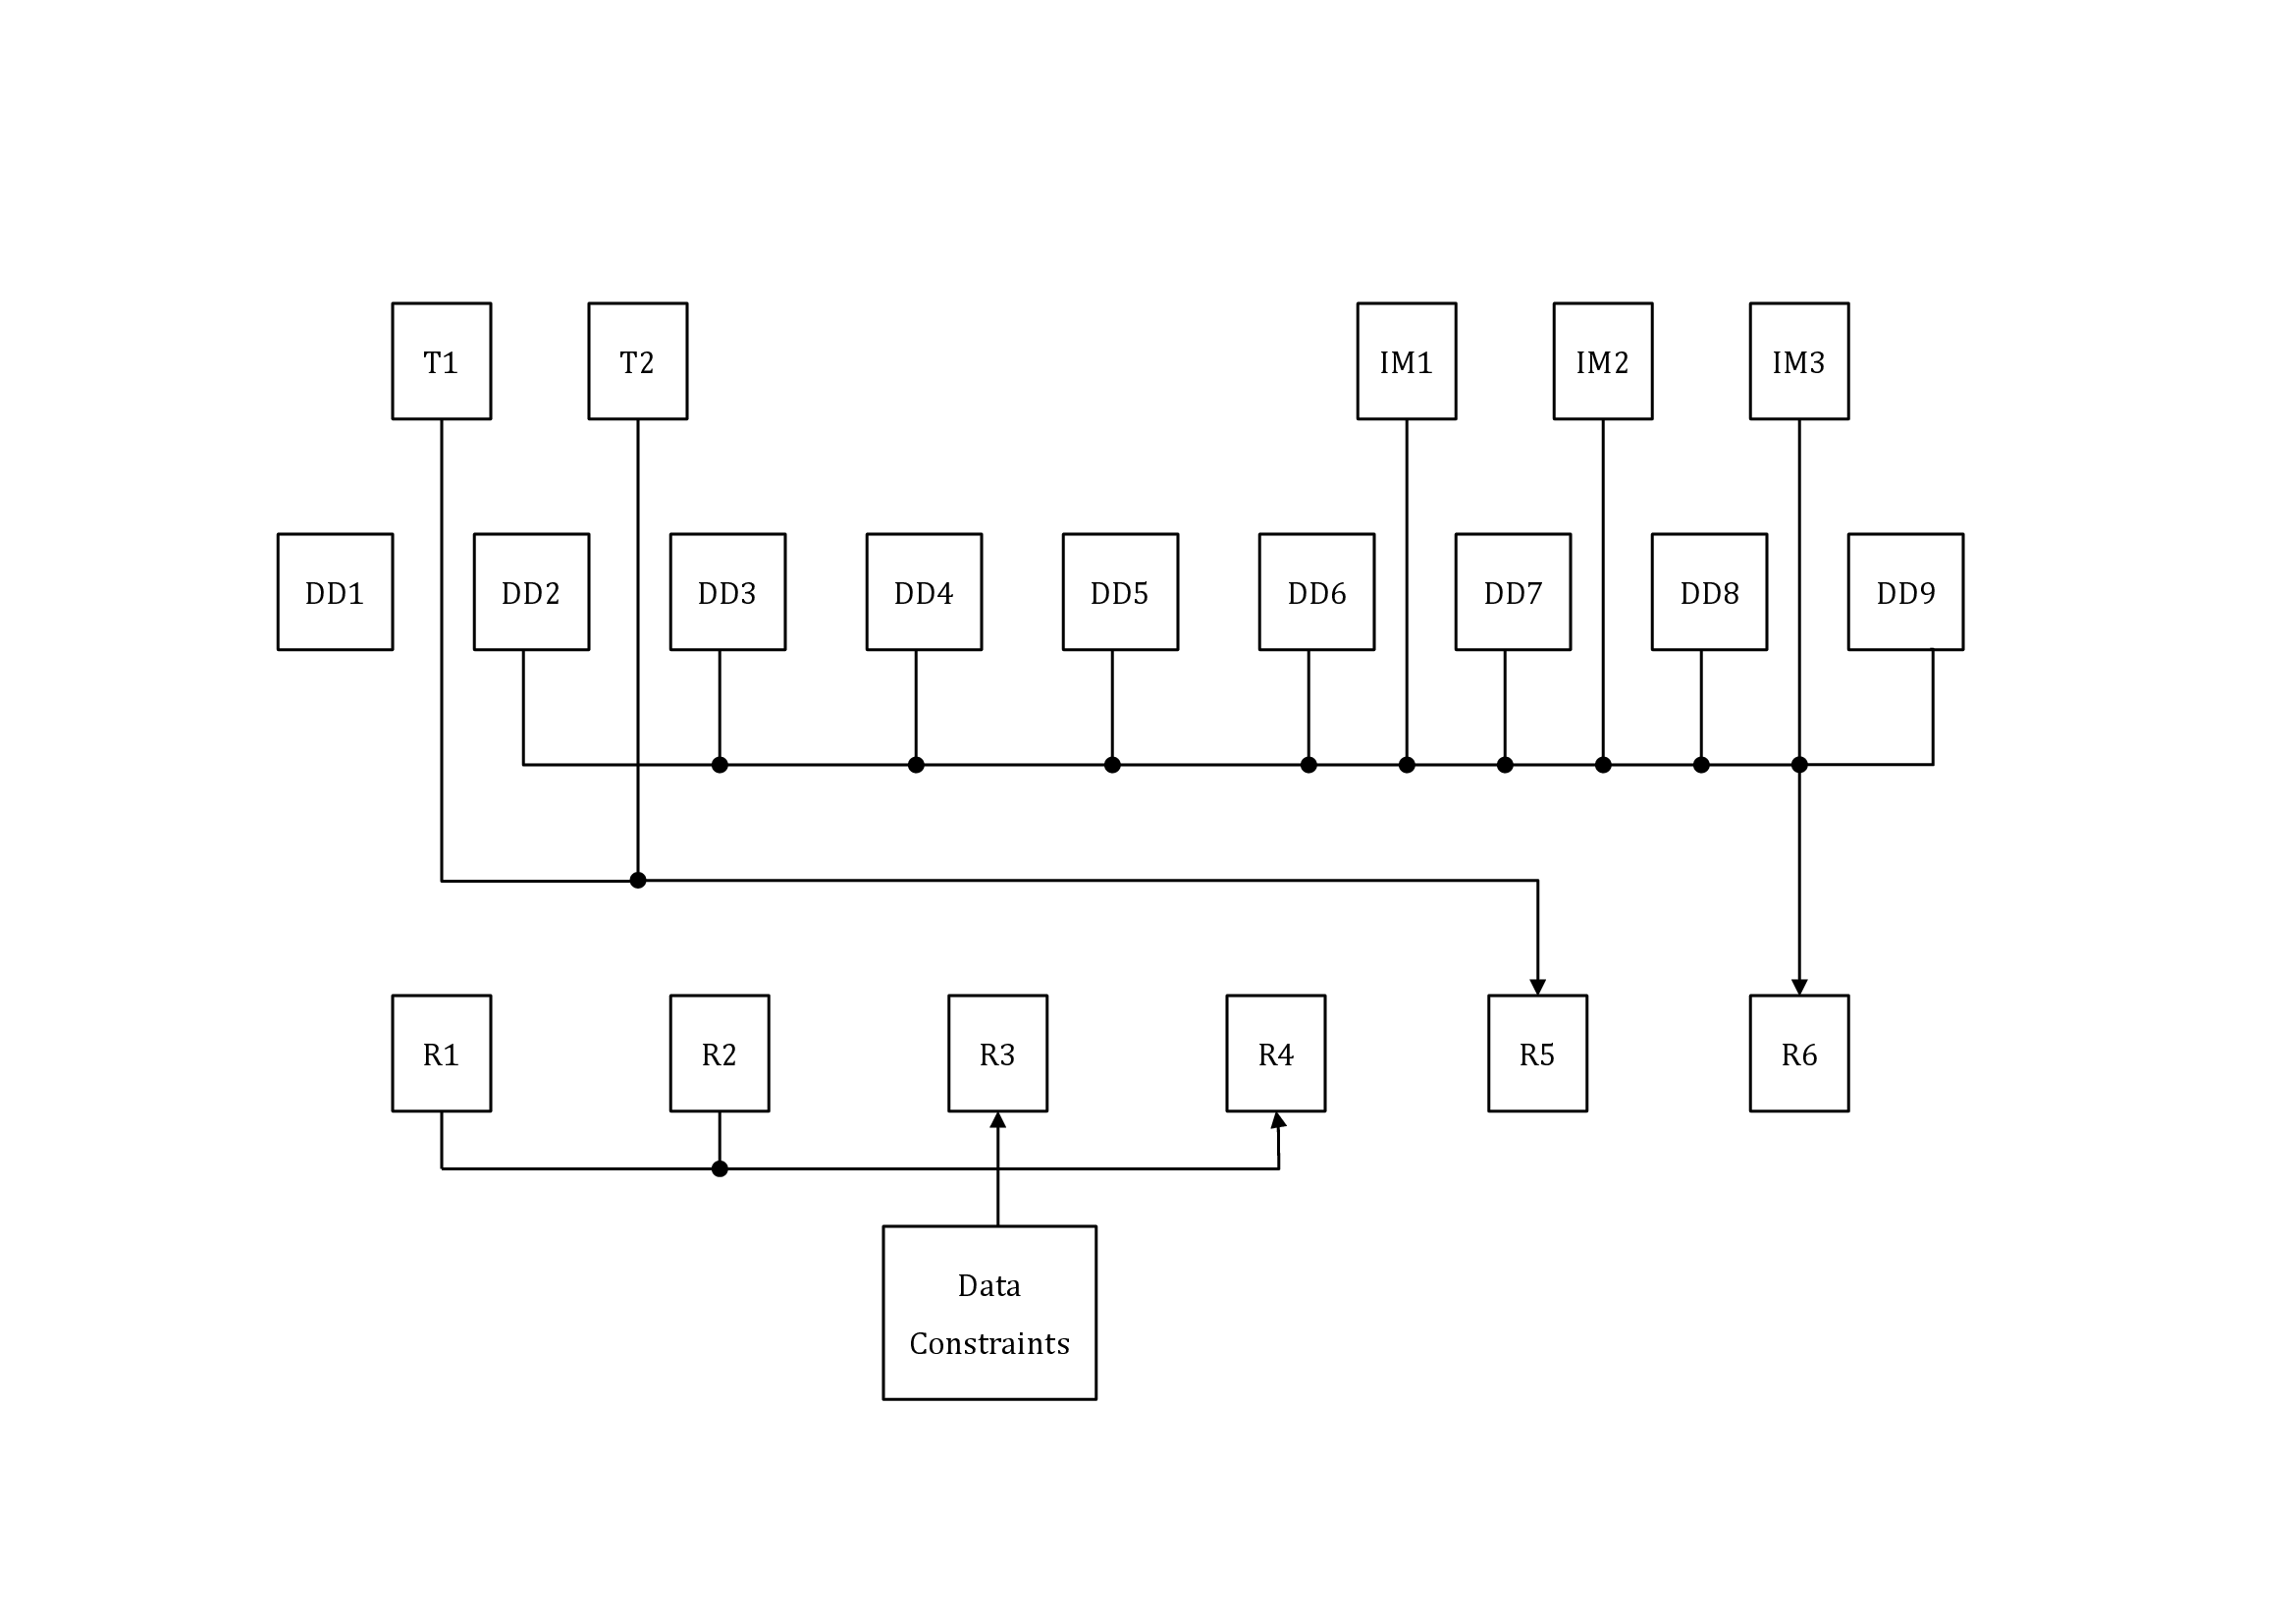
\includegraphics[width=\textwidth]{RTrace.png}
		}
		\caption{\label{Fig_RTrace} Traceability Graph Showing the Connections Between Requirements and Other Items.}
	\end{center}
\end{figure}

\clearpage

\begin{figure}[h!]
	\begin{center}
		%\rotatebox{-90}
		{
			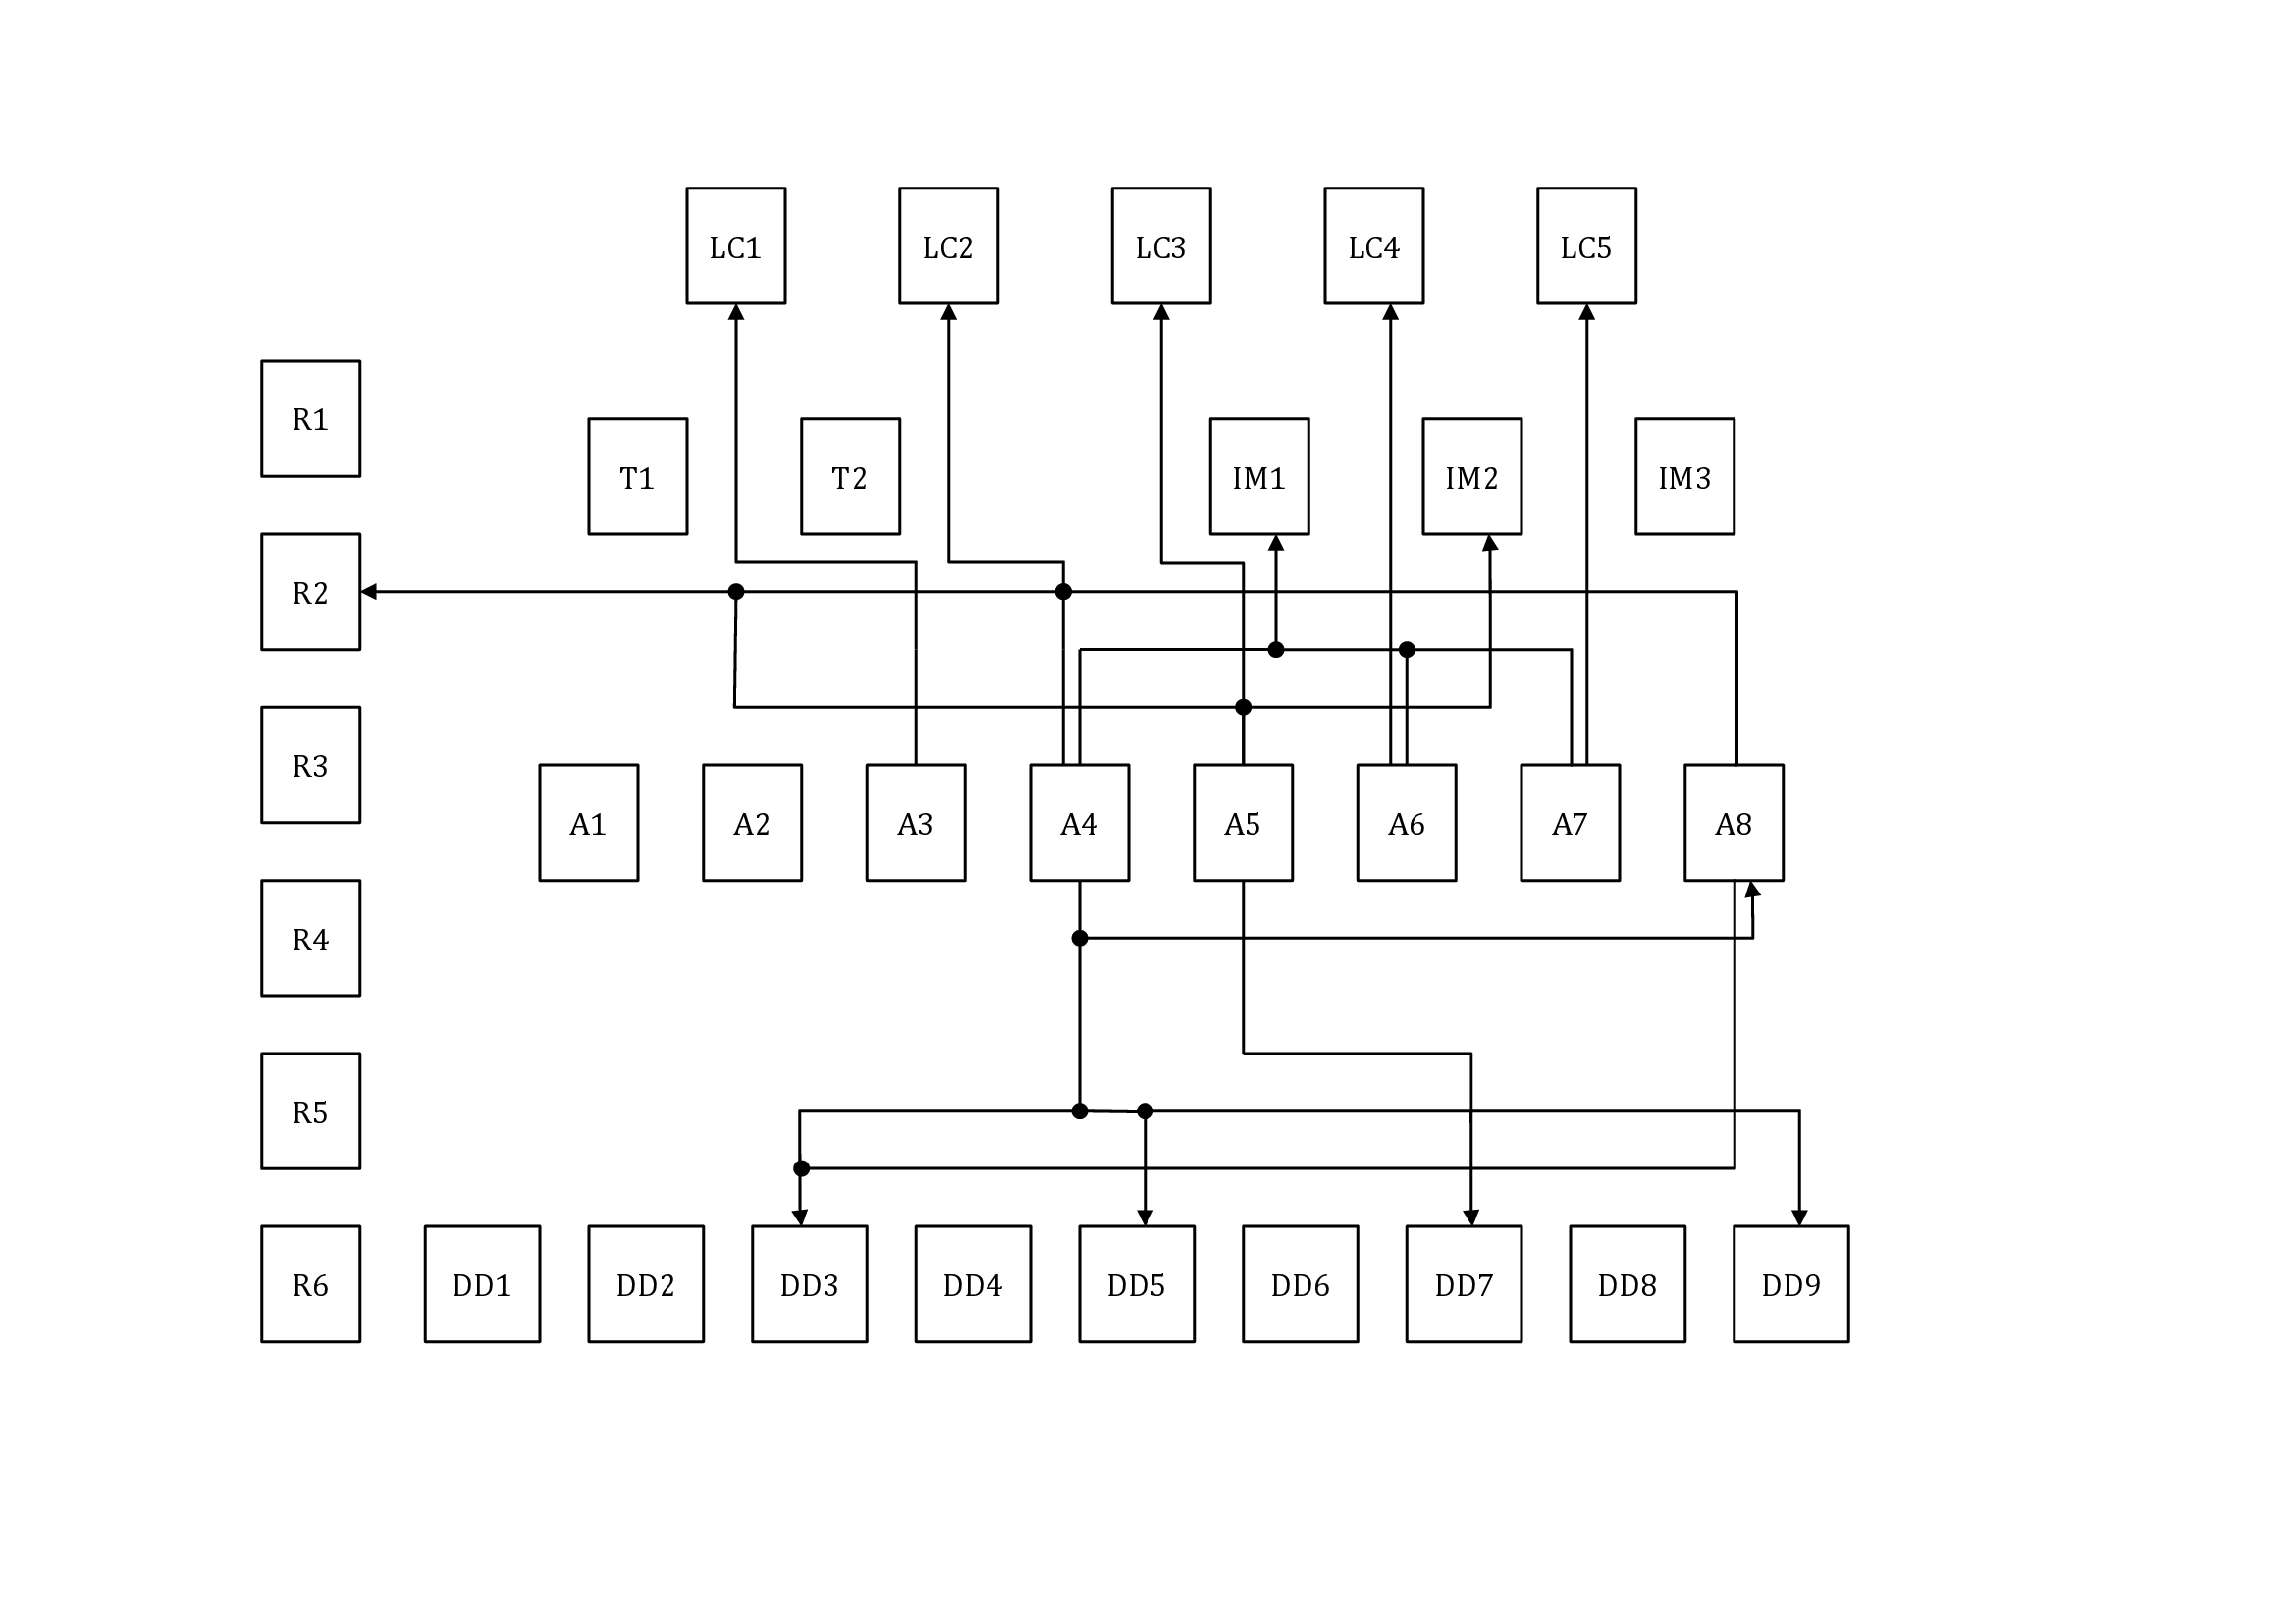
\includegraphics[width=\textwidth]{ATrace.png}
		}
		\caption{\label{Fig_ATrace} Traceability Graph Showing the Connections Between Assumptions and Other Items.}
	\end{center}
\end{figure} 

\section{Values of Auxiliary Constants}
\label{Sec:ValuofAuxiCons}
This section contains the standard values that are used for calculations in
\progname{}.

\begin{longtabu}{l X[l] l l}
\toprule
Symbol & Description & Value & Unit
\\
\midrule
${\text{AR}_{max}}$ & maximum aspect ratio & $5.0$ & --
\\
${d_{max}}$ & maximum value for one of the dimensions of the glass plate & $5.0$ & m
\\
${d_{min}}$ & minimum value for one of the dimensions of the glass plate & $0.1$ & m
\\
$E$ & modulus of elasticity of glass & $7.17\times 10^{7}$ & Pa
\\
$k$ & surface flaw parameter & $2.86\times 10^{-53}$ & $\frac{\text{m}^{12}}{\text{N}^{7}}$
\\
LSF & load share factor & $1$ & --
\\
$m$ & surface flaw parameter & $7$ & $\frac{\text{m}^{12}}{\text{N}^{7}}$
\\
${\text{SD}_{max}}$ & maximum stand off distance permissible for input & $130.0$ & m
\\
${\text{SD}_{min}}$ & minimum stand off distance permissible for input & $6.0$ & m
\\
${t_{d}}$ & duration of load & $3$ & s
\\
${w_{max}}$ & maximum permissible input charge weight & $910.0$ & kg
\\
${w_{min}}$ & minimum permissible input charge weight & $4.5$ & kg
\\
\bottomrule
\caption{Auxiliary Constants}
\label{Table:AuxiCons}
\end{longtabu}

\bibliographystyle{ieeetr}
\bibliography{../../refs/References}

\section{Appendix}

This appendix holds the graphs (Figure~\ref{Fig_ASTM_F2248-09} and
Figure~\ref{ASTM_F2248-09_BeasonEtAl}) used for interpolating values needed in
the models.

\begin{figure}[h!]
 \begin{center}
 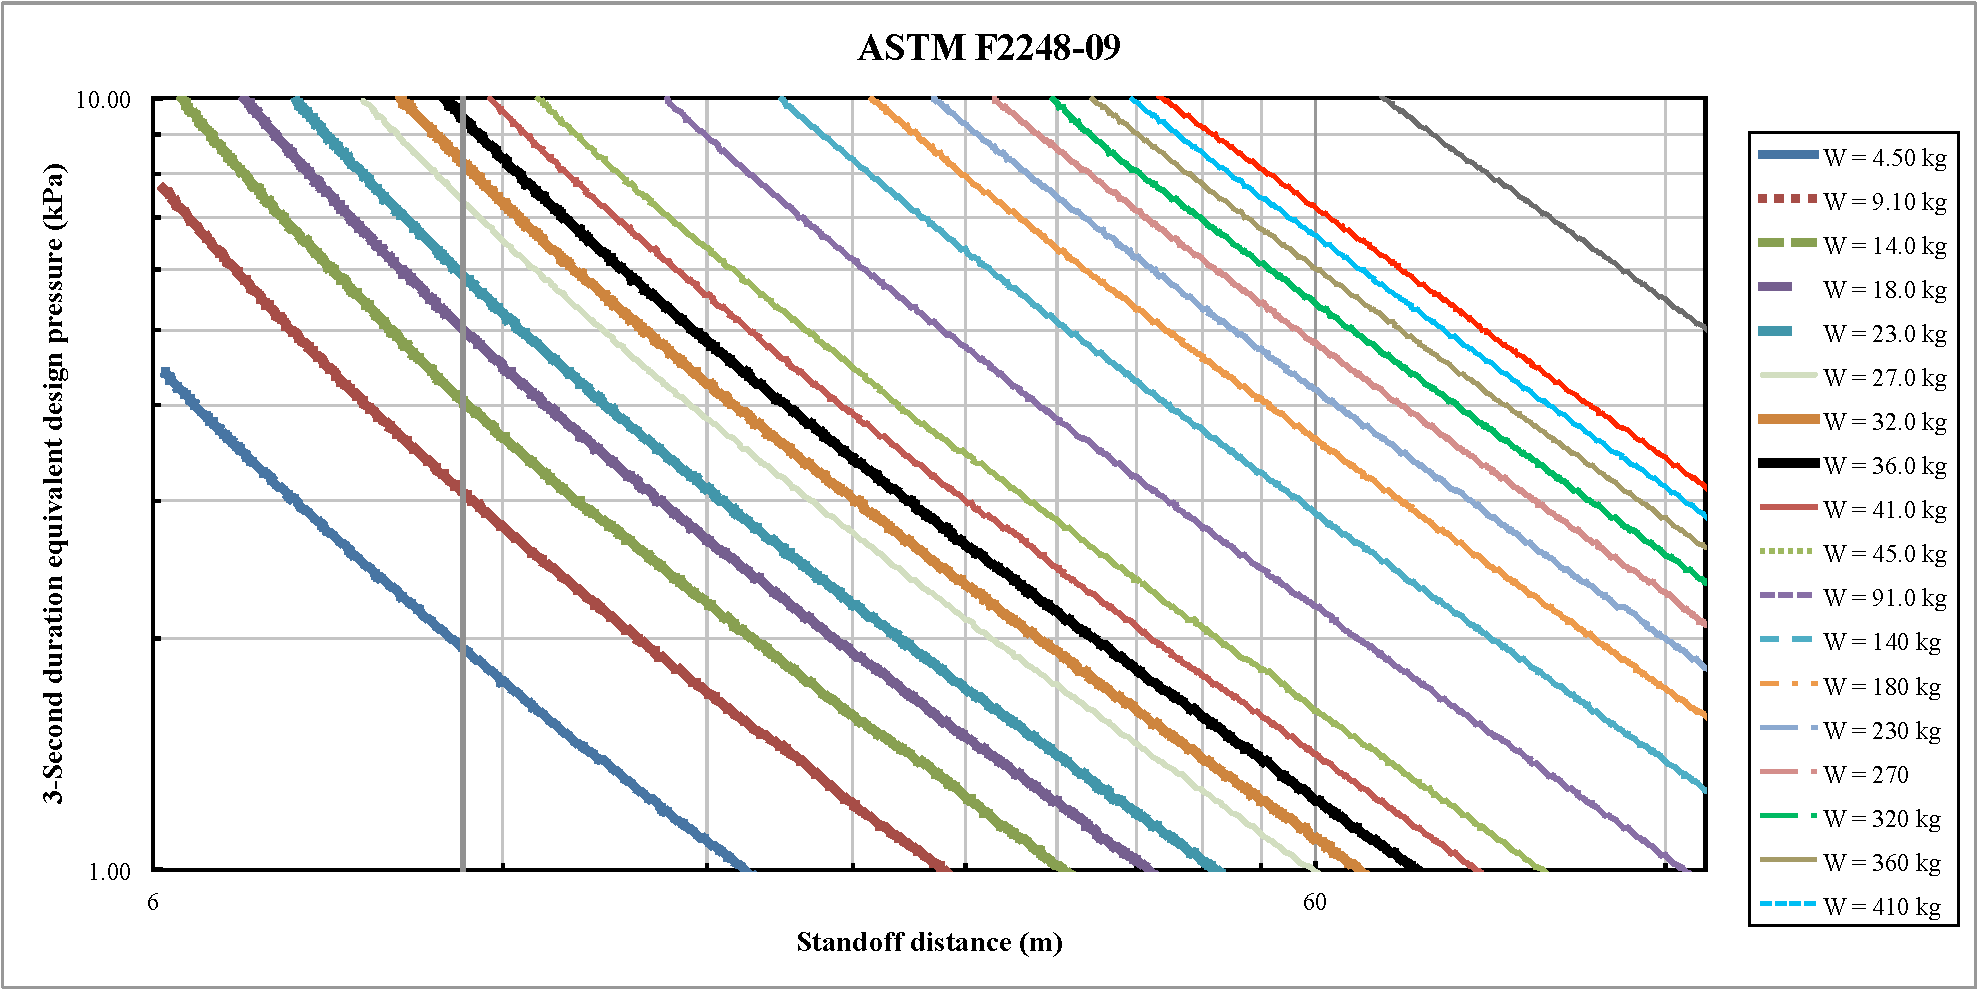
\includegraphics[scale=0.5]{ASTM_F2248-09.pdf}
 \caption{3 second equivalent pressure ($q$) versus Stand off distance ($\text{SD}$) versus
   Charge weight ($w$)}
\label{Fig_ASTM_F2248-09}
 \end{center}
 \end{figure}

 \begin{figure}[h!]
 \begin{center}
 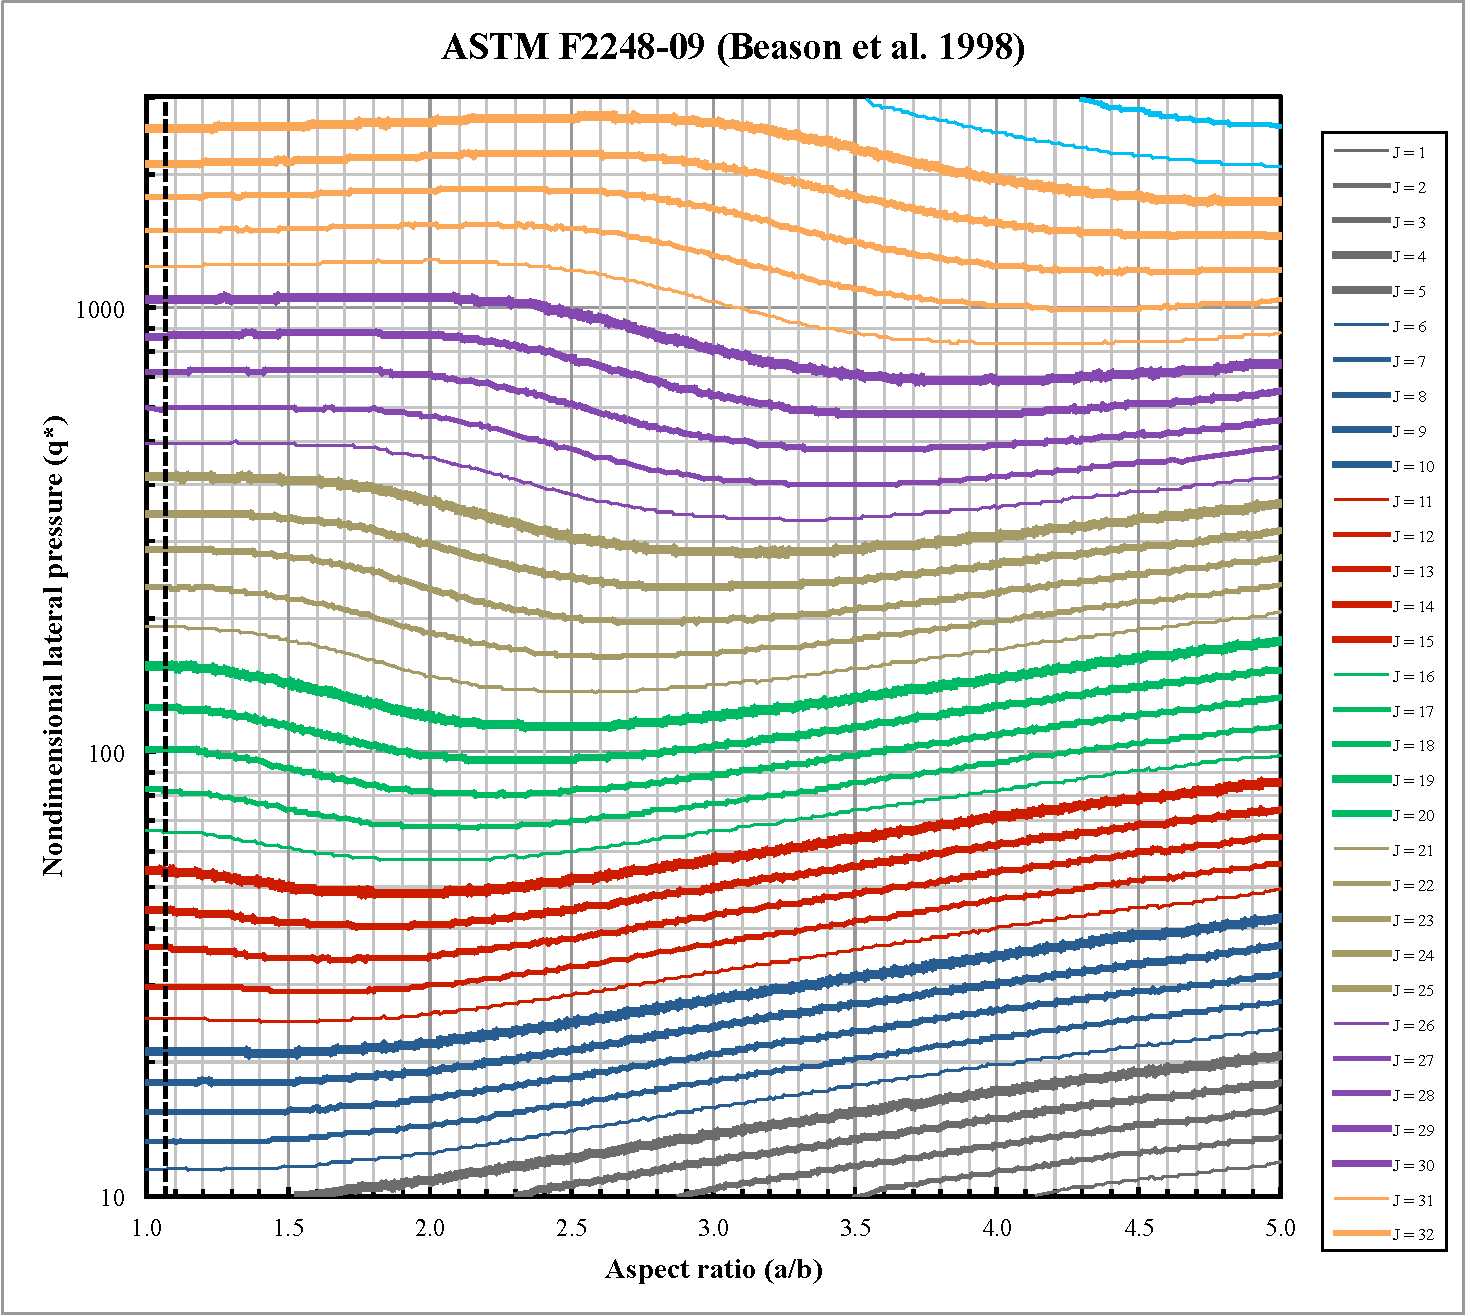
\includegraphics[scale=0.7]{ASTM_F2248-09_BeasonEtAl.pdf}
 \caption{Non dimensional lateral load ($\hat{q}$) versus Aspect Ratio (AR) versus
   Stress distribution factor (Function) (J)}
\label{ASTM_F2248-09_BeasonEtAl}
 \end{center}
 \end{figure}

\end{document}
